%\documentclass[aps,twocolumn,showpacs,superscriptaddress]{revtex4}
\documentclass[aps,showpacs,superscriptaddress]{revtex4}
\usepackage[pdftex]{graphicx}   % for figures
\usepackage{epstopdf}
%\usepackage{epsfig}
%draft
\usepackage{dcolumn}
\usepackage{bm}	
\usepackage{ textcomp }
\usepackage{amsmath}			% Mode math\ufffdmatique
\usepackage{amsfonts}			% Polices math\ufffdmatiques
\usepackage{amssymb}			% Symboles math\ufffdmatiques
\usepackage{latexsym}			% Symboles math\ufffdmatiques avanc\ufffds
\usepackage{color}
%%%%%%%%%%%%%% For submission %%%%%%%%%%%
%  \renewcommand{\baselinestretch}{2} 
%%%%%%%%%%%%%%%%%%%%%%%%%%%%%%%%%%%%%%%%%
\begin{document}
\title{Supplementary information for "Untangling resistive and collisionless electron filamentation instabilities in dense plasmas over large spatial-temporal scales"}

\author{C. Ruyer}\email{charles.ruyer@cea.fr}
\affiliation{LULI - CNRS, Ecole Polytechnique, CEA : Universit\'e Paris-Saclay ; UPMC Univ Paris 06  : Sorbonne Universit\'es - F-91128 Palaiseau cedex, France}\affiliation{SLAC National Accelerator Laboratory, Sand Hill Road, Menlo Park, California, USA}
\affiliation{CEA, DAM, DIF, F-91297 Arpajon, France}
\author{S. Bolanos }
\affiliation{LULI - CNRS, Ecole Polytechnique, CEA : Universit\'e Paris-Saclay ; UPMC Univ Paris 06  : Sorbonne Universit\'es - F-91128 Palaiseau cedex, France}
\author{B. Albertazzi}%\email{Bruno.albertazzi@polytechnique.edu}
\affiliation{LULI - CNRS, Ecole Polytechnique, CEA : Universit\'e Paris-Saclay ; UPMC Univ Paris 06  : Sorbonne Universit\'es - F-91128 Palaiseau cedex, France}
\affiliation{ INRS-EMT, Varennes, Qu\'ebec, Canada}

\author{S.N. Chen}
\affiliation{LULI - CNRS, Ecole Polytechnique, CEA : Universit\'e Paris-Saclay ; UPMC Univ Paris 06  : Sorbonne Universit\'es - F-91128 Palaiseau cedex, France}
\affiliation{Institute of Applied Physics, 46 Ulyanov Street, 603950 Nizhny Novgorod, Russia}
\author{P. Antici}
\affiliation{ INRS-EMT, Varennes, Qu\'ebec, Canada}
\author{J. B\"oker}
\affiliation{Institut f\"ur Laser-und Plasmaphysik, Heinrich-Heine-Universit\"at, D\"usseldorf, Germany}
\author{V. Dervieux}
\affiliation{LULI - CNRS, Ecole Polytechnique, CEA : Universit\'e Paris-Saclay ; UPMC Univ Paris 06  : Sorbonne Universit\'es - F-91128 Palaiseau cedex, France}
\affiliation{CEA, DAM, DIF, F-91297 Arpajon, France}
\author{ L. Lancia}
\affiliation{LULI - CNRS, Ecole Polytechnique, CEA : Universit\'e Paris-Saclay ; UPMC Univ Paris 06  : Sorbonne Universit\'es - F-91128 Palaiseau cedex, France}
\affiliation{Dept. SBAI, Universita di Roma ``La Sapienza'', Via A. Scarpa 14 00181 Rome, Italy}
\author{M. Nakatsutsumi}
\affiliation{LULI - CNRS, Ecole Polytechnique, CEA : Universit\'e Paris-Saclay ; UPMC Univ Paris 06  : Sorbonne Universit\'es - F-91128 Palaiseau cedex, France}
\author{L. Romagnani}
\affiliation{LULI - CNRS, Ecole Polytechnique, CEA : Universit\'e Paris-Saclay ; UPMC Univ Paris 06  : Sorbonne Universit\'es - F-91128 Palaiseau cedex, France}
\author{R. Shepherd}
\affiliation{LLNL, Livermore, United States}
\author{M. Swantusch}
\affiliation{Institut f\"ur Laser-und Plasmaphysik, Heinrich-Heine-Universit\"at, D\"usseldorf, Germany}
\author{M. Borghesi}
\affiliation{School Physics and Astronomy, The Queen's University, Belfast, United Kingdom}
\author{O. Willi}
\affiliation{Institut f\"ur Laser-und Plasmaphysik, Heinrich-Heine-Universit\"at, D\"usseldorf, Germany}
\author{H. P\'epin}
\affiliation{ INRS-EMT, Varennes, Qu\'ebec, Canada}
\author{M. Starodubtsev}
\affiliation{Institute of Applied Physics, 46 Ulyanov Street, 603950 Nizhny Novgorod, Russia}
\author{M. Grech}
\affiliation{LULI - CNRS, Ecole Polytechnique, CEA : Universit\'e Paris-Saclay ; UPMC Univ Paris 06  : Sorbonne Universit\'es - F-91128 Palaiseau cedex, France}
\author{C. Riconda}
\affiliation{LULI - CNRS, Ecole Polytechnique, CEA : Universit\'e Paris-Saclay ; UPMC Univ Paris 06  : Sorbonne Universit\'es - F-91128 Palaiseau cedex, France}
\author{L. Gremillet}\email{laurent.gremillet@cea.fr}
\affiliation{CEA, DAM, DIF, F-91297 Arpajon, France}
\author{J. Fuchs}\email{julien.fuchs@polytechnique.edu}
\affiliation{LULI - CNRS, Ecole Polytechnique, CEA : Universit\'e Paris-Saclay ; UPMC Univ Paris 06  : Sorbonne Universit\'es - F-91128 Palaiseau cedex, France}
\affiliation{Institute of Applied Physics, 46 Ulyanov Street, 603950 Nizhny Novgorod, Russia}

\begin{abstract}
\end{abstract}
\maketitle
\renewcommand\thefigure{S\arabic{figure}}    
\section{Hot electron profile after irradiation of a thin foil by a high-intensity laser  }

\begin{figure*}
\centerline{
\begin{tabular}{ccc}
 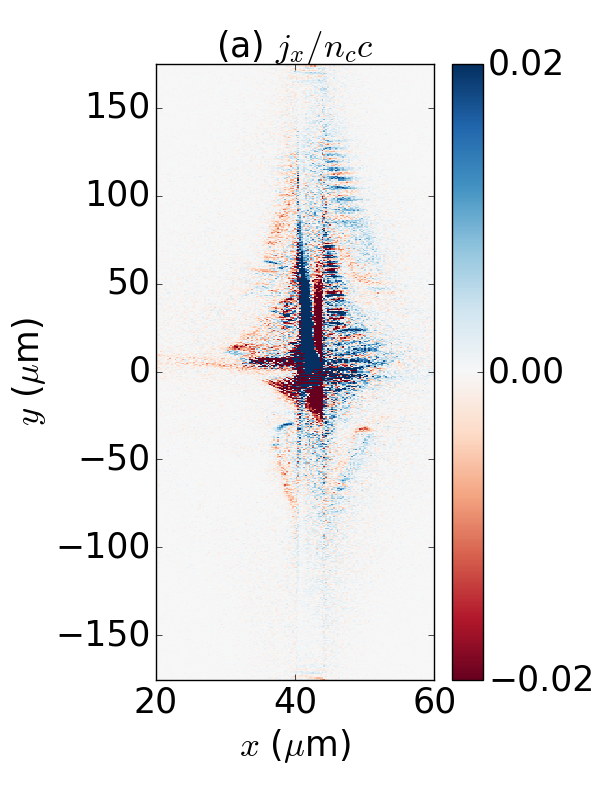
\includegraphics[width=0.33\textwidth]{ix_t104000_nat.png} 
 &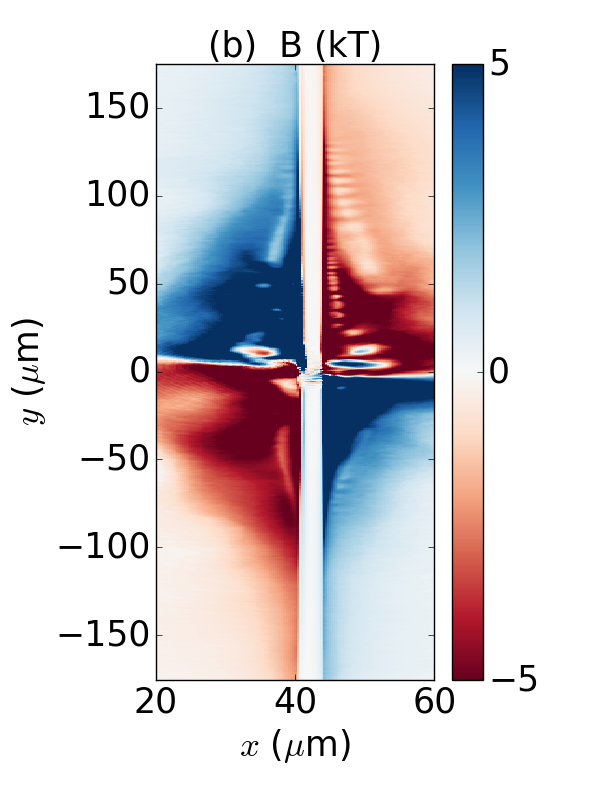
\includegraphics[width=0.33\textwidth]{Bz_t104000_nat.png} 
 &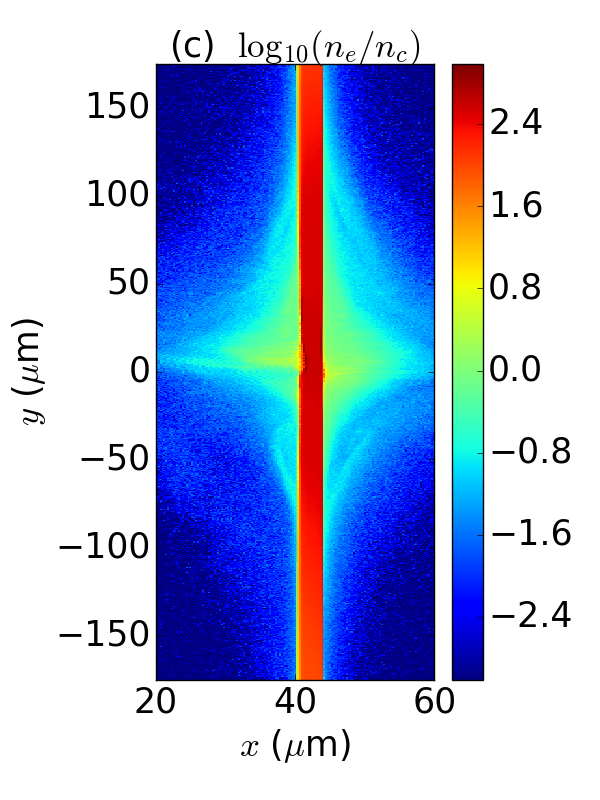
\includegraphics[width=0.33\textwidth]{ne_t104000_nat.png} \\
 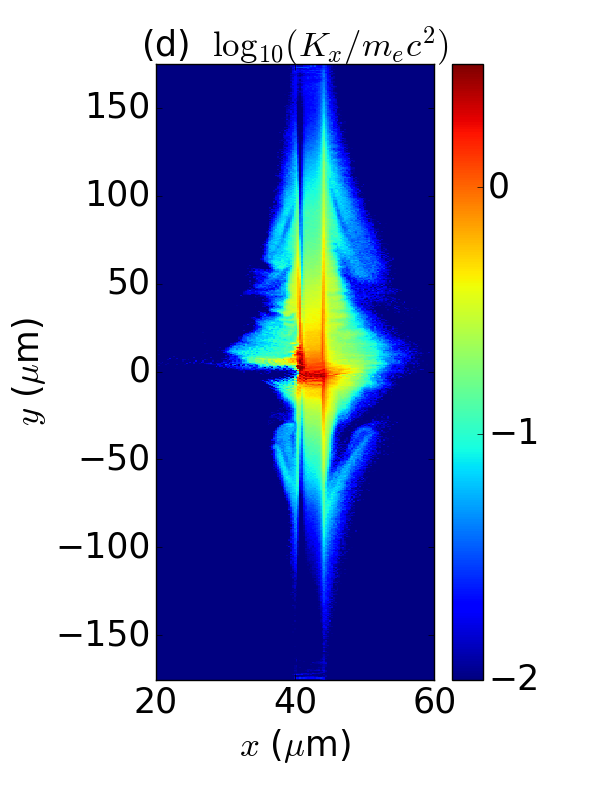
\includegraphics[width=0.33\textwidth]{Kx_t104000_nat.png} 
 &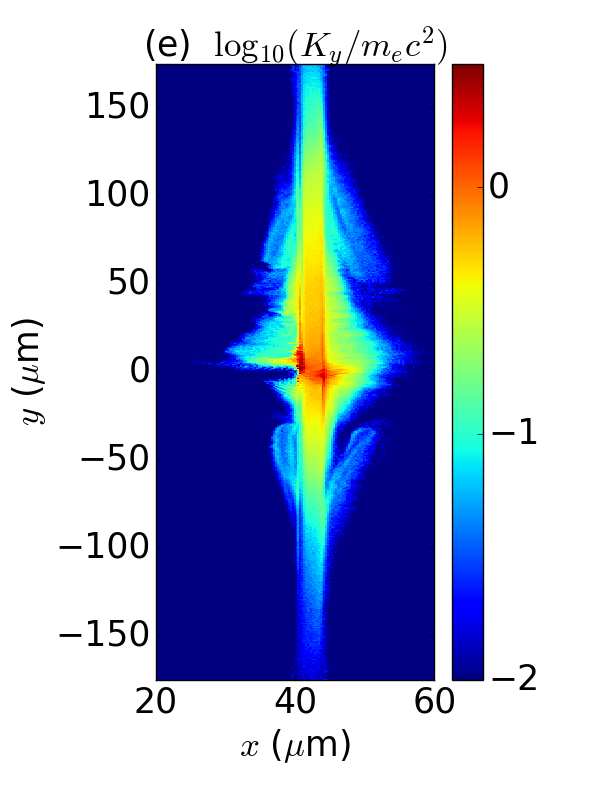
\includegraphics[width=0.33\textwidth]{Ky_t104000_nat.png} 
 &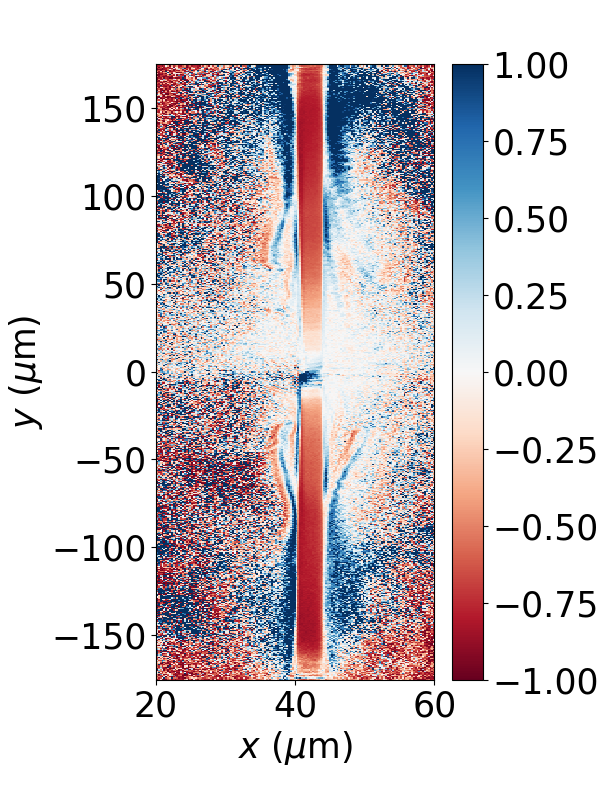
\includegraphics[width=0.33\textwidth]{a_t104000_nat.png} 
\end{tabular}} 
\caption{\label{fig:PIC_las} 
Total $x$-component current (a), magnetic field (b), electron density (c),  in the full PIC simulation of a $3\, \mu$m aluminum foil irradiated by a high intensity laser at $1.4$ ps.
(d,e) Hot electrons $x$ and $y$-aligned momentum flux, (respectively $K_x$ and $K_y$) averaged over the electrons of energy larger than 100 eV.
(f) Hot electron (i.e. energy larger than $100$ eV) anisotropy, $K_x/K_y -1$.
}
\end{figure*}
\begin{figure}[tbh!]
\centerline{
\begin{tabular}{c}
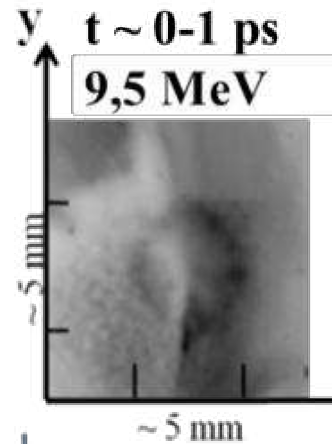
\includegraphics[scale=0.5]{RCF_1ps_Al.png}\\
\end{tabular}}
\caption{\label{fig:rcf_supp} Early time proton radiograph for an aluminum $3\, \mu$m-thick foil. The laser pulse comes from the right side and is focused at the central region of the radiograph at the center of the large circular feature that is induced by the surface Biermann-Battery field \cite[]{RSI_Albertazzi_2015}. The scale refers to the plane of the RCF.
}
\end{figure}

Figures \ref{fig:PIC_las}(a-f) illustrate at 1.4 ps our large scale full PIC 2D simulation of an aluminum foil irradiated by a  temporally Gaussian laser beam of  FWHM $690$ fs and maximum intensity $3.5 \times 10^{19}$ W.cm$^{-2}$ that reached the target at 1.03 ps on the left simulation boundary. The spatial profile is Gaussian with a $6\, \mu$m FWHM focused on the aluminum $3\,\mu$m-thick target (see section methods for details). 
As in the experiment, the beam inclination is of  $-30$ degrees compared to the target normal and propagates from the bottom-left corner of the simulation toward the center of the foil.
Figures \ref{fig:PIC_las}(a,b) show that self generated magnetic fluctuations associated with a current is triggered in the expanding plasma [see Fig. \ref{fig:PIC_las}(c)] at $x\sim 50 \, \mu$m and far from the focal spot $y>75\, \mu$m. These fields develop preferentially in the upper part of the simulation compared to where the laser points to, suggesting that the  hot electron plays a crucial role in triggering the instability. The initial directionality of these fluctuations is consistent with the early time experimental observation shown in Fig. \ref{fig:rcf_supp}.
Indeed, the modulations revealed by the probing protons are seen on the left side of the laser irradiation spot, when the laser arrives on the target from the right side of this image. 
Afterward, as illustrated in Fig. 2 of the main paper, the distribution of the spot-like structures   becomes independent of the laser orientation, \emph{i.e.} the structures are observed all over the target surface.

The $(x,y)$-aligned momentum flux  averaged over the electrons of energy larger than 100 eV is  illustrated  in Figs.  \ref{fig:PIC_las}(d,e) after the laser-energy deposition, showing that the hot electron pressure is larger in the y direction than normally to the target plane, except at the center of the foil (at the irradiation region), where the hot electron pressure remains isotropic. 
The ratio between $K_y$ and $K_x$ of Fig. \ref{fig:PIC_las}(f) demonstrates that  the anisotropy polarity is reversed  in the expanding plasma outside the foil and for $x \le 50\, \mu$m, we have $K_y < K_x$ consistently with the anisotropy expected from the Weibel-type instabilities responsible of the field and magnetic field observed in Figs.  \ref{fig:PIC_las}(a,b).

A y-lineout of the hot electrons density (of energy larger than 100 eV) at the end of the simulation ($t=1.44$ ps)   is illustrated in  Fig. \ref{fig:nhcut} and presents a maximum density of $n_h\sim 5 \times 10^{21}$ cm$^{-3}$ and spatial extension of roughly $R_0 \sim 30\, \mu$m. These parameters have been used as initial hot electron parameters for the PIC-MHD simulation addressing the late time electron dynamics in the resistive medium.
\begin{figure}[tbh!]
\centerline{
\begin{tabular}{c}
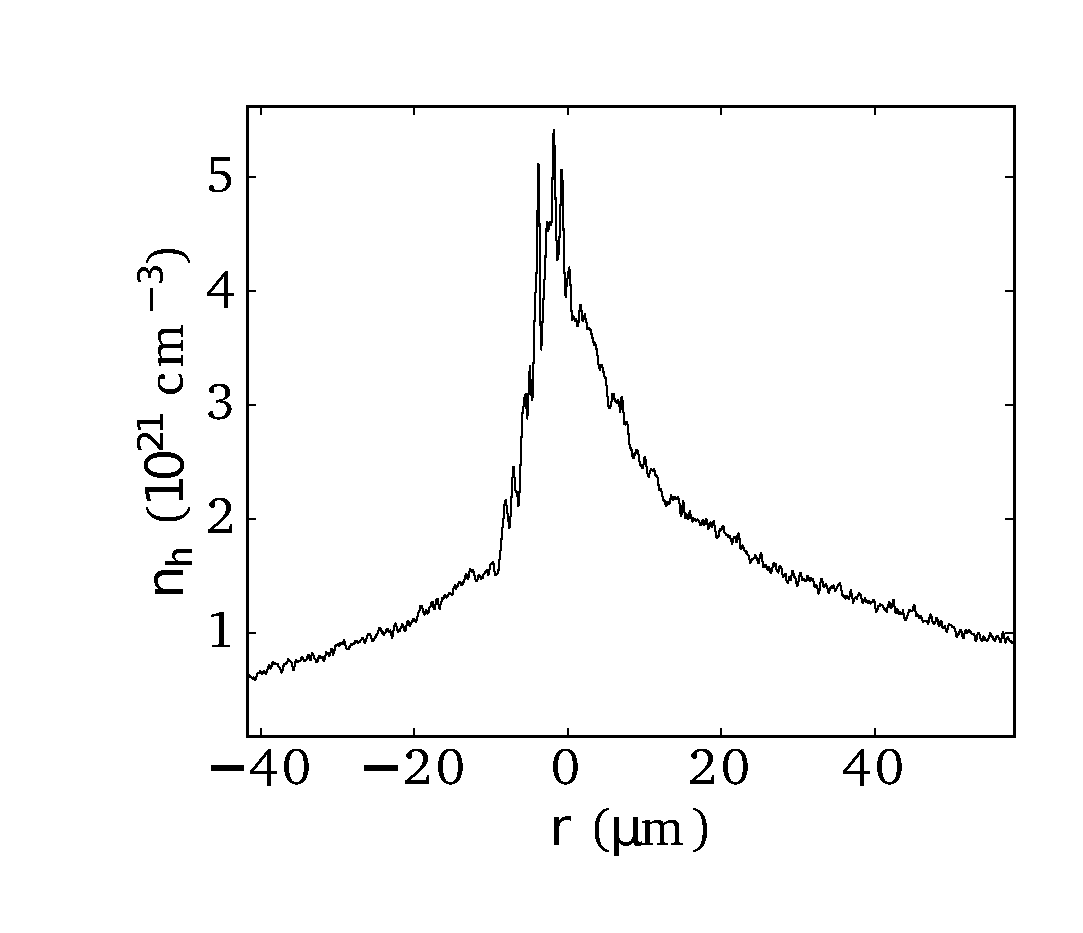
\includegraphics[scale=0.5]{nh_comPICMHD_t104000.eps}
\end{tabular}}
\caption{\label{fig:nhcut} Lineout of the hot ($>100$ eV) density at the center of the dense foil in the full PIC 2D simulation at $1.44$ ps .
}
\end{figure}


\section{Resistive Dispersion relation}
We derive here the electromagnetic dispersion relation of a homogeneous and resistive plasma in the presence of a hot-electron population. The hot electrons ($h$-subscript) and the ions ($i$-subscript) will be both  described by a multi-Maxwellian distribution, while the cold electrons ($c$-subscript) that ensure charge and current neutralization will be assumed to fulfill a generalized Ohm's law. Introducing the first-order perturbation of the  current, $\mathbf{j}^{(1)} = \mathbf{j}_i^{(1)} +\mathbf{j}_h^{(1)}+\mathbf{j}_c^{(1)}$, we will express the ion and hot electron contributions, $\mathbf{j}_i^{(1)}$ and $\mathbf{j}_h^{(1)}$, by linearizing the Vlasov-Maxwell equations.
We will here assume  $\mathbf{j}_h^{(1)} +\mathbf{j}_i^{(1)} =- \sigma \mathbf{E} +\mu_0^{-1}\nabla \times \mathbf{B} - \epsilon_0 \partial_t \mathbf{E}$ where $\sigma$, $\mathbf{E}$, $\mathbf{B}$, $\mu_0$, and $\epsilon_0$ are the electrical conductivity,  electric field, magnetic field, vacuum permeability and permittivity respectively.
We then obtain 
\begin{equation}\label{eq:rose}
i \sum_{s =h,i} \omega_{ps}^2 \int d\mathbf{p} \frac{\nabla_pf_s}{\omega -\mathbf{k}\cdot\mathbf{v}}\cdot \left( 1 +\mathbf{v}\times \frac{\mathbf{k}}{\omega} \times \right)\mathbf{E}
+ i\omega \left( 1 + \frac{\sigma }{i\omega \epsilon_0}+ \frac{\mathbf{k}}{\omega}\times \frac{\mathbf{k}}{\omega} \times \right)\mathbf{E} =0 \, .
\end{equation}
The first hand side of the above equation corresponds to the hot electron and ion current from the linearized Vlasov equation. The second hand side is the generalized Ohms'law.
The determinant of Eq. \eqref{eq:rose} can be expressed as a function of the  collisionless  plasma susceptibility tensor, $\epsilon =  1 + \sum_{s = i,h} \chi_s\omega_{ps}^2/\omega^2$, where $\omega_{ps}$ is the plasma frequency of the $s$-species.

Although  derived in a Cartesian geometry, we will assume that this dispersion relation can still be applied locally, far from the irradiated region. At a distance of $\sim 100\, \mu$m away from the hot spot, the hot electrons drift in the radial direction and are cooler in the poloidal direction than in the x direction. We will therefore model the hot electrons by the following Maxwellian distribution function 
\begin{equation}\label{eq:distrib}
f_h(v_r, v_\phi,v_x) \propto \exp\left[ -\frac{m_ev_\phi^2}{2T_\phi} -\frac{m_ev_x^2}{2T_x} -\frac{m_e(v_h-v_r)^2}{2T_r} \right]\, .
\end{equation}
We introduced the poloidal, $x$ and radial temperature and drift velocity, $T_\phi$, $T_x$, $T_r$, $v_r$ respectively. 
Note that, we make use of  $\phi$, $x$ and $r$ only to ease the comparison with the experimental geometry, the dispersion relations are Cartesian.

%In the non-relativistic regime the dispersion relation associated with the three possible planes are independent. 
We will now consider the case where the wavevector lies in the $(r,\phi)$-plane. 
The determinant of Eq.~\eqref{eq:rose} gives
\begin{equation}\label{eq:dispe0}
\left(\omega^2 \epsilon_{rr} - k_\phi^2c^2 +\frac{i\omega}{\tau_E}\right)
\left(\omega^2 \epsilon_{\phi\phi} - k_r^2c^2 +\frac{i\omega}{\tau_E}\right)
-\left(\omega^2 \epsilon_{r\phi} - k_\phi k_rc^2\right)^2 = 0 \, ,
\end{equation}
where use has been made of $\tau_E = \epsilon_0/\sigma$.

\subsection{Case of a wavevector perpendicular to the drift velocity (poloidal)}

Solving the dispersion relation for a wavevector perpendicular to the drift velocity corresponds, in the experiment, to a poloidal wavevector [instability seen in Fig.~4(a) at $r = 200\, \mu$m]: $k = k_\phi$. 
Plugging $k = k_\phi$ into Eq. \eqref{eq:dispe0} gives
\begin{equation}\label{eq:dispe}
\left(\omega^2 \epsilon_{rr} - k_\phi^2c^2 +\frac{i\omega}{\tau_E}\right)
\left(\omega^2 \epsilon_{\phi\phi} +\frac{i\omega}{\tau_E}\right)
-\omega^4 \epsilon_{r\phi}^2 = 0 \, ,
\end{equation}
In this case, the bi-Maxwellian susceptibility tensor verifies \cite[]{POP_Ruyer_2015}
\begin{align}
 \epsilon &=  1 + \sum_{s = i,h}\frac{\omega_{ps}^2}{\omega^2}  \chi_s\, , \label{eq:eps}\\
  \chi_{rr} &= -1  + \frac{m_sv_s^2 + T_{sr} }{T_{s\phi}} [1+\xi_s\mathcal{Z}(\xi_s) ]\, \label{eq:chixx},\\
  \chi_{\phi\phi} &=-\xi^2 \partial_\xi\mathcal{Z}(\xi_s) \, ,\\
  \chi_{r\phi} & =  -v_s\sqrt{\frac{m_s}{2T_{s\phi}}} \xi_s \partial_\xi \mathcal{Z}(\xi_s)  \label{eq:chixy}\, ,\\
  \xi_s  &= \frac{\omega }{k_\phi} \sqrt{\frac{m_s}{2T_{s\phi}}}\label{eq:xi} \, .
\end{align}
The approximate analytical resolution of the dispersion relation can be achieved with a Taylor development of the dispersion function $\mathcal{Z}(\xi_s)$. For $\vert \xi_h \vert\gg 1$
\begin{align}
\mathcal{Z}(\xi_h) & =  i\pi^{1/2}(1-\xi_h^2) -2\xi_h +\frac{4}{3}\xi_h^3 + \mathrm{O}(\xi_h^5) \label{eq:taylor1} \, ,\\
d_{\xi_h} \mathcal{Z}(\xi_h)  &= -2\xi_h -2i\pi^{1/2}\xi_h^2 +4\xi_h^3+ \mathrm{O}(\xi_h^5)\label{eq:taylor2} \, .
\end{align}
Assuming immobile ions and introducing  $K_{sx} = m_sv_s^2 + T_{sx}$, the third order Taylor development of \eqref{eq:chixx}-\eqref{eq:chixy} gives
\begin{align}
  \chi_{rr} &\simeq -1  + \frac{K_{hx} }{T_{hy}} + \frac{K_{hx} }{T_{hy}} ( i\pi^{1/2}\xi_h -2\xi_h^2 -i\pi^{1/2}\xi_h^3) \, ,\\
  \chi_{\phi\phi} &\simeq2\xi_h^2+ 2i\pi^{1/2}\xi_h^3 \, ,\\
  \chi_{r\phi} & \simeq  -v_h\sqrt{\frac{m_s}{2T_{hy}}} (2\xi_h + 2i\pi^{1/2}\xi_h^2 -4\xi_h^3) \, .
\end{align}
To third order in $\omega$, Eq.~$\eqref{eq:dispe}$ can be recast as a second order polynomial equation 
\begin{align}
&\mathcal{A}\omega^2 +\mathcal{B}\omega +\mathcal{C} = 0\, , \label{eq:dispepoloidal} \\
\mathcal{A}& =\frac{2i}{\tau_E} + i\sqrt{\frac{\pi}{2}}\frac{K_{hr} }{T_{h\phi}}\frac{\omega_{ph}^2}{k_\phi v_{th\phi}} -\frac{i}{\tau_E}\frac{\omega_{ph}^2}{k_\phi^2 v_{th\phi}^2}(a_\phi-1) 
+i\sqrt{\frac{\pi}{2}}\frac{\omega_{ph}^4}{k_\phi^3 v_{th\phi}^3} \frac{T_{hr} }{T_{h\phi}} \label{eq:a} \, , \\
\mathcal{B} & =   - \sqrt{\frac{\pi}{2}}\frac{K_{hr} }{T_{h\phi}}\frac{\omega_{ph}^2}{k_\phi v_{th\phi} \tau_E}
+\omega_{ph}^2(a_\phi-1)-\omega_{ph}^2 \frac{c^2}{v_{th\phi}^2} -k_\phi^2 c^2 -\frac{1}{\tau_E^2 } 
 + \frac{\omega_{ph}^4}{k_\phi^2 v_{th\phi}^2}\left[(a_\phi-1)- \frac{v_h^2}{2v_{th\phi}^2} \right]  \, , \label{eq:b} \\
\mathcal{C} & =\frac{i}{\tau_E}(\omega_{ph}^2 a_\phi -k_\phi^2c^2 )\label{eq:c}\, , 
\end{align}
where $a_\phi = K_{hr}/T_{h\phi}$ and $v_{th\phi} = \sqrt{T_{h\phi}/m_e}$. 
The above equation gives
\begin{equation}
\omega  = -\frac{\mathcal{B}}{2\mathcal{A}}\left(1\pm \sqrt{1-\frac{4\mathcal{A}\mathcal{C}}{\mathcal{B}^2}} \right)
\label{eq:dispesol}\, .
\end{equation}
In order to apply the above result to the case of the $(\phi,x)$-anisotropy, one just needs to use $v_h = 0$ and replace $r$ by $x$.
\begin{figure*}[ht]
\centerline{
\begin{tabular}{cc}
\multicolumn{2}{c}{Poloidal \emph{vs.} radial anisotropy: $v_h = 100\, \mu\mathrm{m}/1.2\, ps \simeq 0.3c$, $T_r = T_\phi = 50$ keV, $n_h = 2\times 10^{19}$ cc, $T_{c}=50$ eV}\\
(a) $\Gamma(k_y)$&(b)  $\xi_h= \Gamma/k_yv_{thy}$ \\
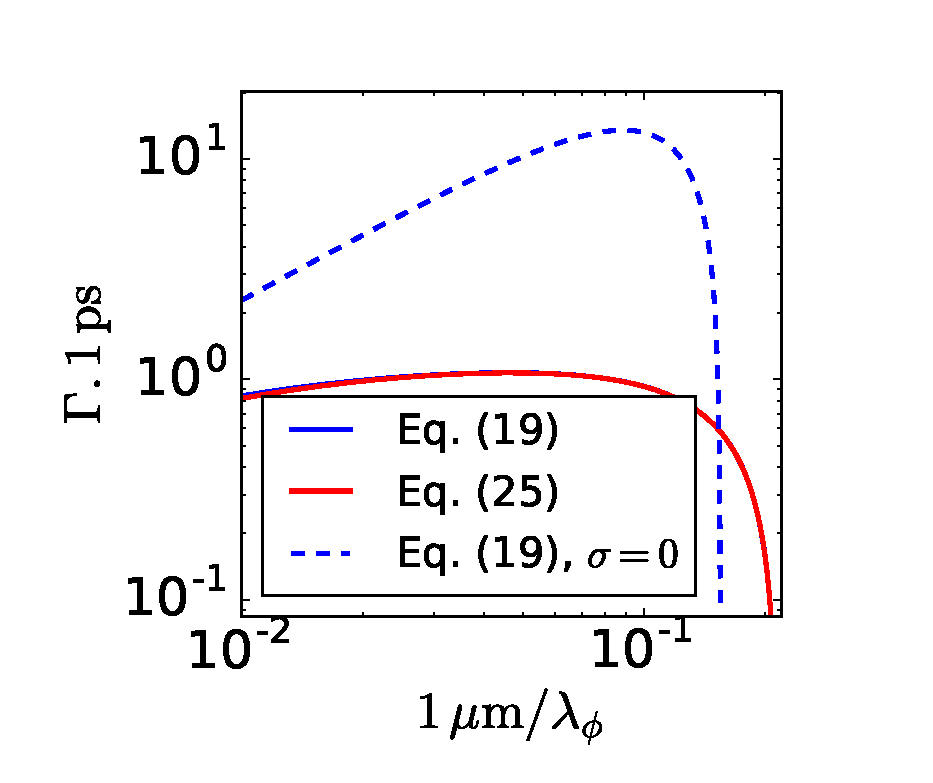
\includegraphics[width=0.33\textwidth]{gamma_ky_ordre3_r_phi_vh.eps} 
 &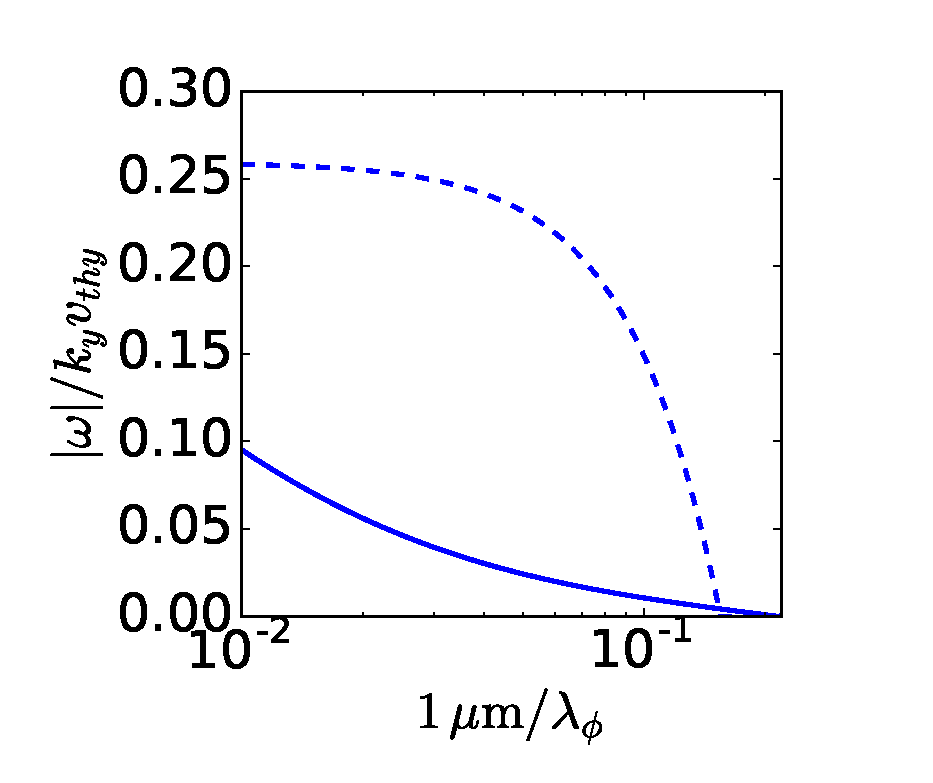
\includegraphics[width=0.33\textwidth]{xi_ky_ordre3_r_phi_vh.eps} \\
\multicolumn{2}{c}{Poloidal \emph{vs.} $x$ anisotropy: $v_h = 0 $, $T_x=0.5$ MeV, $T_\phi = 10$ keV, $n_h = 2\times 10^{19}$ cc, $T_{c}=50$ eV }\\
(c) $\Gamma(k_y)$&(d)  $\xi_h= \Gamma/k_yv_{thy}$ \\
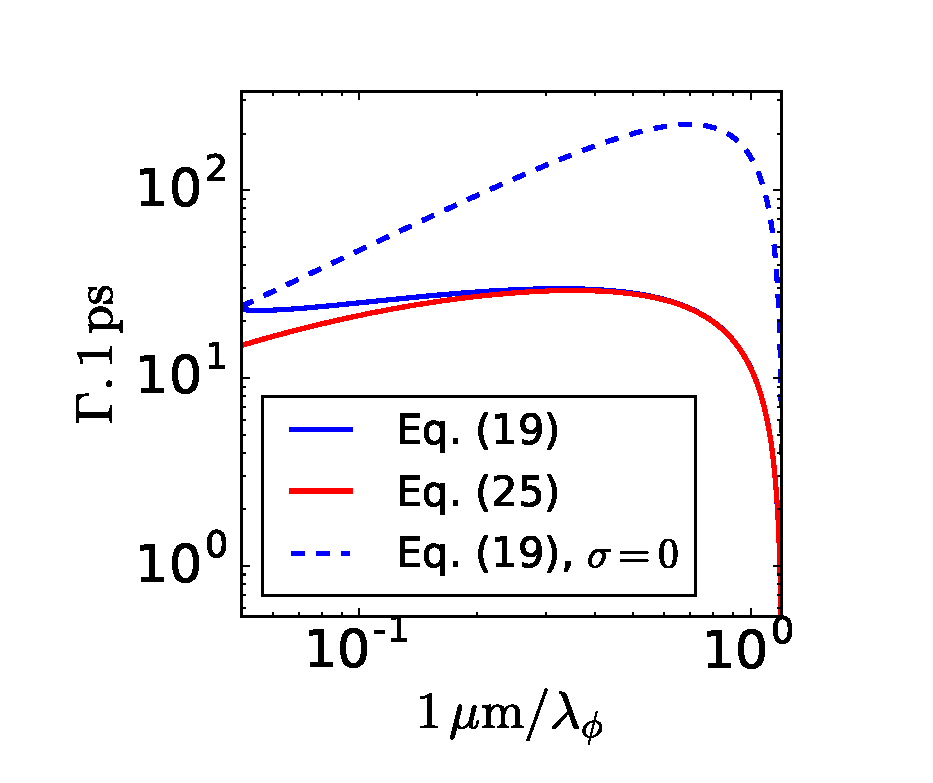
\includegraphics[width=0.33\textwidth]{gamma_ky_ordre3_r_phi.eps} 
 &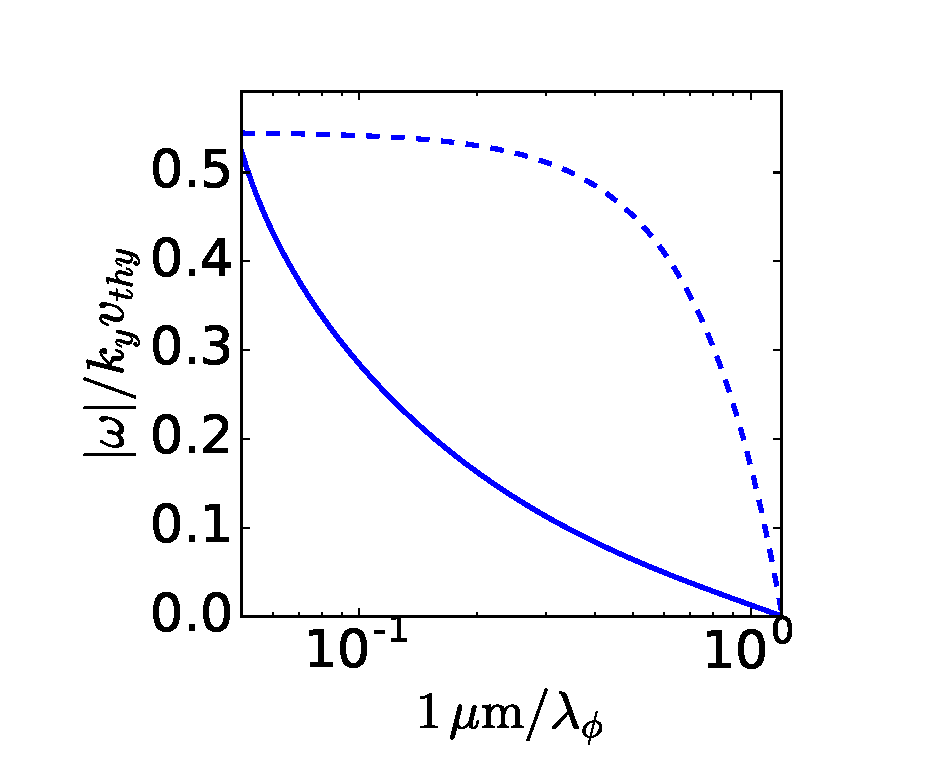
\includegraphics[width=0.33\textwidth]{xi_ky_ordre3_r_phi.eps} \\
\multicolumn{2}{c}{Poloidal \emph{vs.} $x$  anisotropy: $v_h = 0 $, $T_x=0.5$ MeV, $T_\phi = 10$ keV, $n_h = 2\times 10^{19}$ cc, $T_{c}=20$ eV }\\
(e) $\Gamma(k_y)$&(f) $\xi_h= \Gamma/k_yv_{thy}$ \\
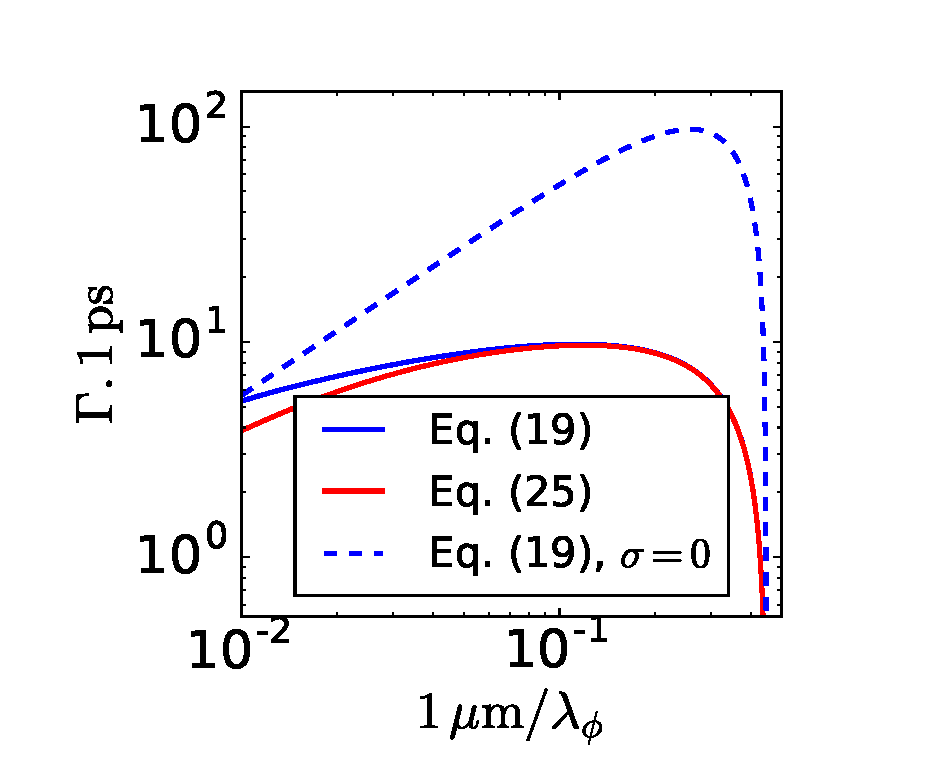
\includegraphics[width=0.33\textwidth]{gamma_ky_ordre3_r_phi_2.eps} 
 &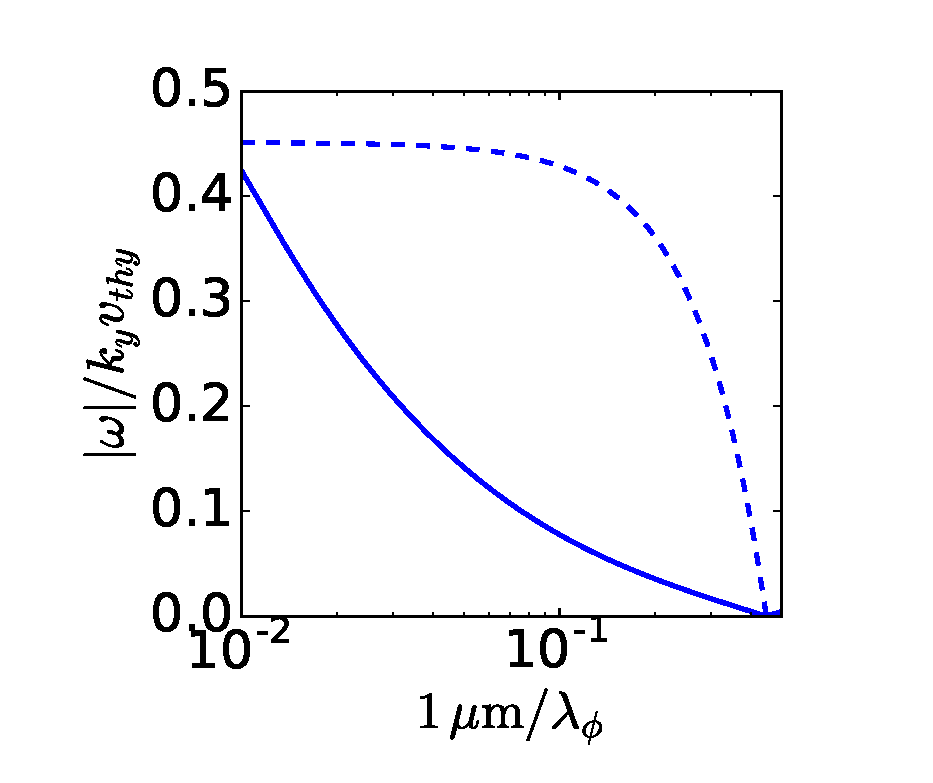
\includegraphics[width=0.33\textwidth]{xi_ky_ordre3_r_phi_2.eps} 
\end{tabular}} 
\caption{\label{fig:gamma_ky} 
(a) Growth rate ($\Gamma$) and Taylor expansion parameter ($\xi_h$) as a function of $k_\phi$ with resistivity (plain line) and without (dashed line).
The conductivity is calculated following Ref.  \cite[]{POP_Perez_2012} with a cold electron temperature of $T_c = 50\,\mathrm{eV}$ corresponding to $Z_\star = 7$. 
}
\end{figure*}

Figures~\ref{fig:gamma_ky}(a,c,e) plot $(r, \phi)$ and $(\phi,x)$ growth rates from the above equations as a function of the wavevector normalized to $1\, \mu$m ($k_yc/\omega_0 = 1\mu\mathrm{m}/\lambda_\phi$) with and without resistivity in plain and dashed lines respectively. 
%The parameters of Figs.~\ref{fig:gamma_ky}(a-d) correspond to the plasma parameters extracted from the region $r\sim 200 \, \mu$m, $t = 3.28$ ps of Fig.~3 (main paper). 
In all cases, the presence of a resistive background electrons significantly decreases the Weibel growth rate (by more than an order of magnitude) and the wavevector of the fastest-growing mode (by a factor $\sim 3$). 
The fastest growing mode is obtained when the pressure anisotropy is carried by the temperature like in Figs.~\ref{fig:gamma_ky}(c,d)  where $v_h = 0$ which demonstrates that the instability of poloidal wavevector is triggered, in our case, by the temperature anisotropy, and not the streaming of particles.
%Note that, although decreased, the resistive Weibel growth rate is still consistent with our experimental results since for Fig.~\ref{fig:gamma_ky}(a), $\Gamma_\mathrm{max}\sim 3\times  10^{-2}\omega_0 \simeq (0.1 \, \mathrm{ps})^{-1}$.
Finally, care has been taken to verify that the argument of the Taylor expansion of Eqs.~\eqref{eq:taylor1}-\eqref{eq:taylor2}, illustrated in Figs. \ref{fig:gamma_ky}(b,d,f),
verifies $\xi_h \lesssim 0.1$ in the region where the growth rate is maximized.

\subsection{Analytical estimates of the dominant mode}

In order to obtain a simple analytical formulation of the dominant mode wavevector and growth rate, we will first only retain the dominant terms of Eqs. \eqref{eq:a}-\eqref{eq:c}. In our system for which $\omega_{ph} \tau_E \ll 1$, we obtain
\begin{align}
\mathcal{A} & \simeq \frac{2i}{\tau_E}  \label{eq:a2} \, , \\
\mathcal{B} & \simeq    - \sqrt{\frac{\pi}{2}}\frac{K_{hr} }{T_{h\phi}}\frac{\omega_{ph}^2}{k_\phi v_{th\phi} \tau_E}
 -\frac{1}{\tau_E^2 }  \, , \label{eq:b2} \\
\mathcal{C} & \simeq \frac{i}{\tau_E}(\omega_{ph}^2 a_\phi -k_\phi^2c^2 )\label{eq:c2}\, , 
\end{align}

Combined with Eq. \eqref{eq:dispesol}, it follows
\begin{equation}
\Gamma_\phi  \simeq \frac{1}{4}  \sqrt{ \left( \sqrt{\frac{\pi}{2}} \frac{\omega_{ph}^2}{k_\phi v_{th,\phi}}a_\phi    + \frac{1}{\tau_E} \right)^2 +  8(\omega_{ph}^2 a_\phi  - k_\phi^2 c^2 )   }  -\frac{1}{4}   \sqrt{\frac{\pi}{2}} \frac{\omega_{ph}^2}{k_\phi v_{th,\phi}}a_\phi    -\frac{1}{4}   \frac{1}{\tau_E}
\label{eq:dispesol2}\, .
\end{equation}

 Solving $\partial_{k_\phi} \Gamma = 0 $ gives the wavevector that maximizes the growth rate and leads to a polynomial equation of the order ten, so that in order to have a tractable estimate, we relate the dominant wavevector $k_\mathrm{max}$ to $k_\star$ which is defined as $\Gamma_\phi (k_\star>0)=0$. We will then relate $k_\mathrm{max}$ to a fraction of $k_\star =  a_\phi^{1/2}\omega_{ph}/c$, giving 
\begin{equation}\label{eq:ksat}
k_\mathrm{max} \simeq 0.5 k_\star = \frac{a_\phi^{1/2}\omega_{ph}}{2c} \, .
\end{equation}
%We therefore deduce the effective growth rate 
%\begin{equation}\label{eq:gf}
%\Gamma_\phi(k_\mathrm{sat})  \simeq \frac{1}{4}  \sqrt{ \left( 2\sqrt{\frac{\pi m_ec^2}{2T_{h0}}} \omega_{ph}a_\phi    + \frac{1}{\tau_E} \right)^2 +  6\omega_{ph}^2 a_\phi   }  -\frac{1}{2}\sqrt{\frac{\pi m_ec^2}{2T_{h0}}} \omega_{ph} a_\phi   -\frac{1}{4}   \frac{1}{\tau_E}
%\end{equation}
Figs. \ref{fig:gamma_ky}(a,c,e)  illustrate successful comparisons between the growth rate of Eq. \eqref{eq:dispesol} (blue plain line) and its approximation, Eq. \eqref{eq:dispesol2}  (red plain line) for  solid-density plasma relevant for our study. In particular, the maximum of the growth rate is well reproduced by our approximated formula.

\section{Spatio-temporal evolution of the plasma parameters}
We will here examine the hot-electron plasma parameters and their evolution as a function of space and time. 

\subsection{hot electron dynamics in an insulator and in a conductor-type target} 
Figures \ref{fig:nt}(a-f) present the radial profiles of the hot and cold electron ($\ge 100$ eV) parameters for the two cases, $\log(\Lambda)=2$ and $20$. 
It is instructive to assess that no significant difference is observed between these two cases regarding $n_h$, $v_r$, $T_x$ and $K_r$ (\emph{i.e.} the hot electron density, radial drift velocity, $x$-aligned temperature and radial averaged momentum flux). Only the poloidal temperature [Fig. \ref{fig:nt}(e)] presents a slightly larger temperature for the insulator ($\log(\Lambda)=20$)  than the conductor ($\log(\Lambda)=2$) in the region $r\gtrsim 50\, \mu$m. 
This suggests that the hot electron dynamics, for fast enough particles, weakly depends on the background electrons at early times.
However, Fig. \ref{fig:nt}(b) shows that the cold electron ($\lesssim 100$ eV) density is larger in a high resistivity than in a low resistivity target. Indeed, a larger resistive current implies a larger amount of impact ionization and therefore a larger cold electron density, consistently with our PIC-MHD simulations. 

Regarding the second moments of the hot electron distribution, 
the   poloidal  temperature verifies $T_\phi\sim 10$ keV and  is  smaller than the corresponding radial momentum flux and the $x$-aligned temperature ($K_r\gtrsim 70$ keV and $T_x\gtrsim 100$ keV),  as evidenced by Figs. \ref{fig:nt}(d-f) for $r\gtrsim 50\, \mu$m. This configuration is therefore unstable regarding the resistive filamentation instability with a wavevector aligned with the poloidal direction, as derived in Sec. II of this document and illustrated in Fig. 3(e) of the main paper.

\subsection{Hot electrons density evolution}
Let us assume that the hot electrons, initially located in a circle of radius $R_0$, have a density of $n_{h0}$ and temperature $T_{h0}$. The cold electron  population initially verifies charge neutrality and has a temperature $T_{c0}$.
A simple way to estimate the time-decreasing density of the fast electrons, $n_h(r,t)$, as they expand radially, is by expressing particle number conservation over the hot electron light cone.
For an initial electron  deposition radius $R_0$, the electrons will drift radially, so that after a time t, the fast electrons will be  filling a surface $\propto ( R_0 + v_{h0}t)^D$, where D is the number of dimensions in the foil plane and $(T_{h0}/m_e)^{1/2}= v_{h0}\sim c$.
The size of the target in the expanding direction follows $\propto (L+c_st)^\delta$ where $c_s$, $L$ and $\delta$ are  the hot electron sound speed, the target initial thickness and the number of dimension in the expanding direction, respectively. 
For a homogeneous repartition of the hot electrons over their light cone, the conservation of the particle number gives
\begin{equation} \label{eq:nt}
n_h(r,t)  = n_{h0} \left( \frac{R_0}{R_0 + v_{h0}t } \right)^D \left( \frac{L}{L + c_{s}t } \right)^\delta  H \left( 1 + \frac{v_{h0}t-r}{R_0} \right) \, ,
\end{equation}
where $H$ is the step function.
Fig.  \ref{fig:n_param} presents the  homogeneous  hot electron density profile extracted from one  MHD-PIC simulations at two times  and is found to be in agreement with our estimates.
The temporal evolution of the spatially averaged hot electron density (normalized to $n_{h0}$) is illustrated in Fig. \ref{fig:n_param}(a) for various PIC MHD simulations (for $D=2$, $\delta=1$). Although the numerical density evolution seems somewhat slower than our predictions, due to the use of   $(T_{h0}/m_e)^{1/2} \simeq c$ for simplicity, a fair agreement is obtained.
\begin{figure}[ht]
\centerline{$T_{h0} = 1\,\mathrm{MeV}$, $T_{c0} = 50\,\mathrm{eV}$, $n_{h0} = 5 \times 10^{21}\,\mathrm{cm}^{-3}$ and $R_0 = 30\,\mu\mathrm{m}$}
\centerline{\begin{tabular}{ccc}
(a) $n_h$ & (b) $n_{ec}$ &(c)  $v_r$  \\
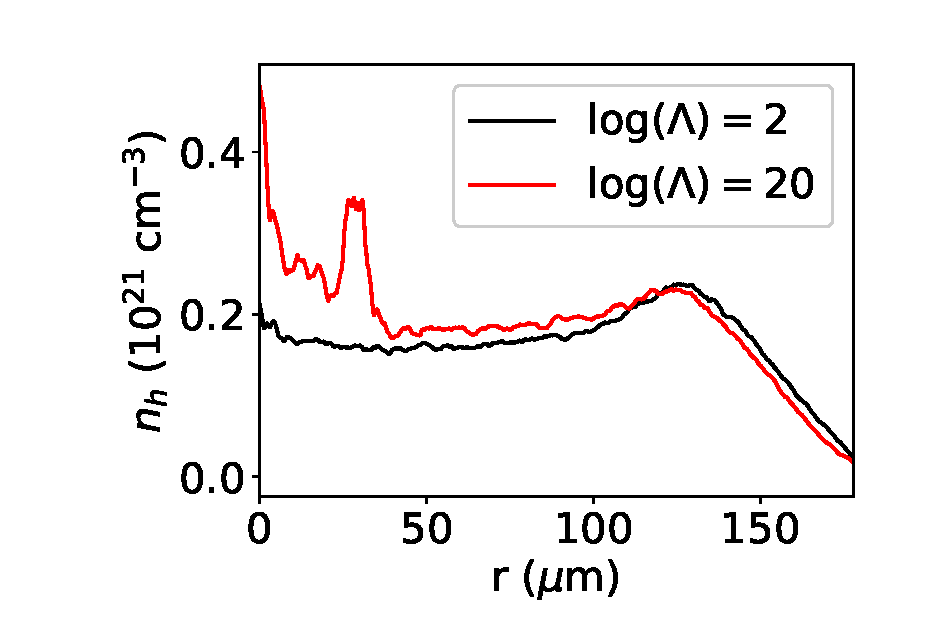
\includegraphics[width=0.32\textwidth]{nh_MHD_sup.eps}&
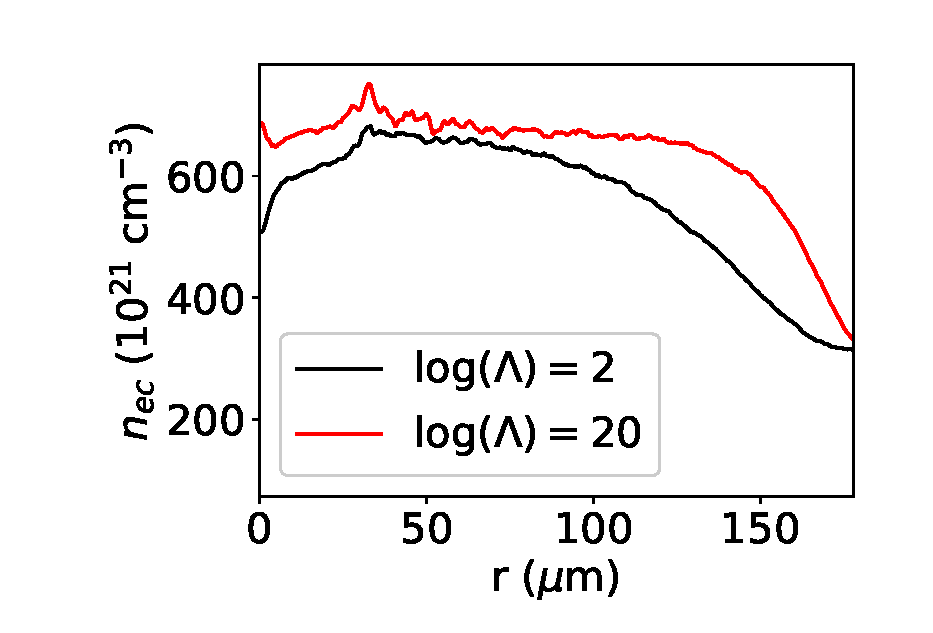
\includegraphics[width=0.32\textwidth]{nec_MHD_sup.eps}&
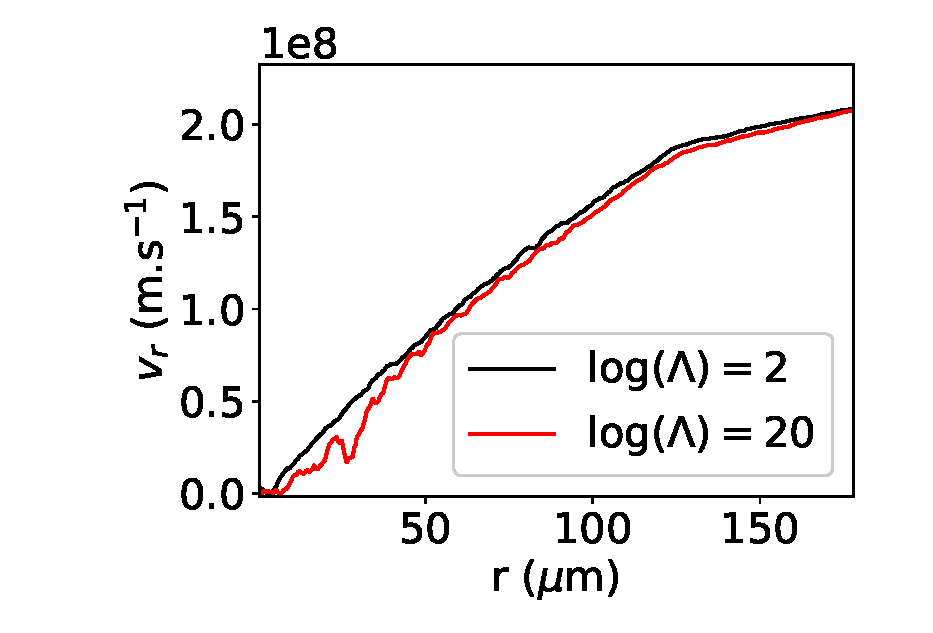
\includegraphics[width=0.33\textwidth]{vr_MHD_sup.eps}\\
(d) $T_x$  &(e) $T_\phi$& (f) $K_r=\frac{m_ev_r^2}{2}+T_r$ \\
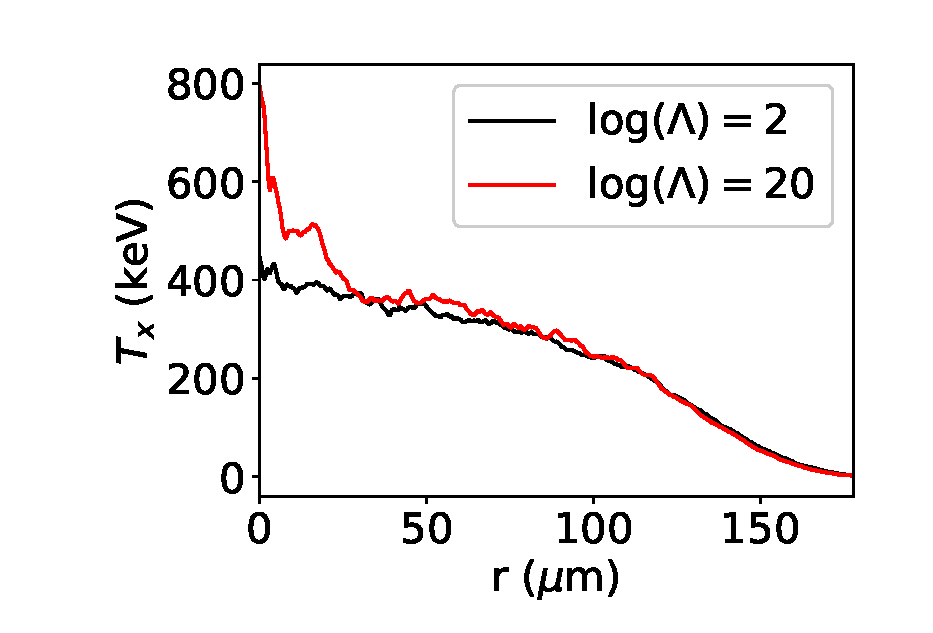
\includegraphics[width=0.32\textwidth]{Tx_MHD_sup.eps} &
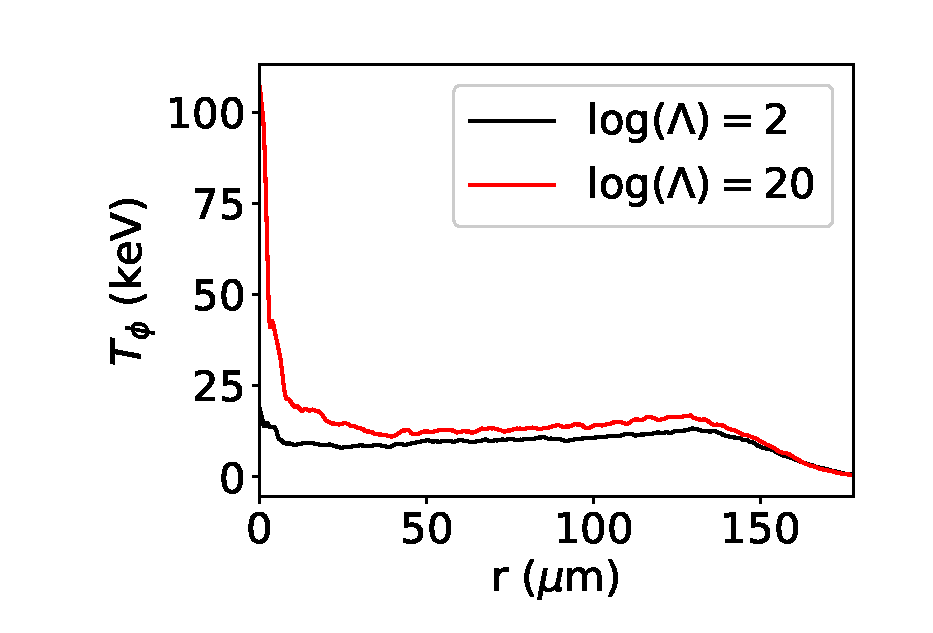
\includegraphics[width=0.32\textwidth]{Tp_MHD_sup.eps}&
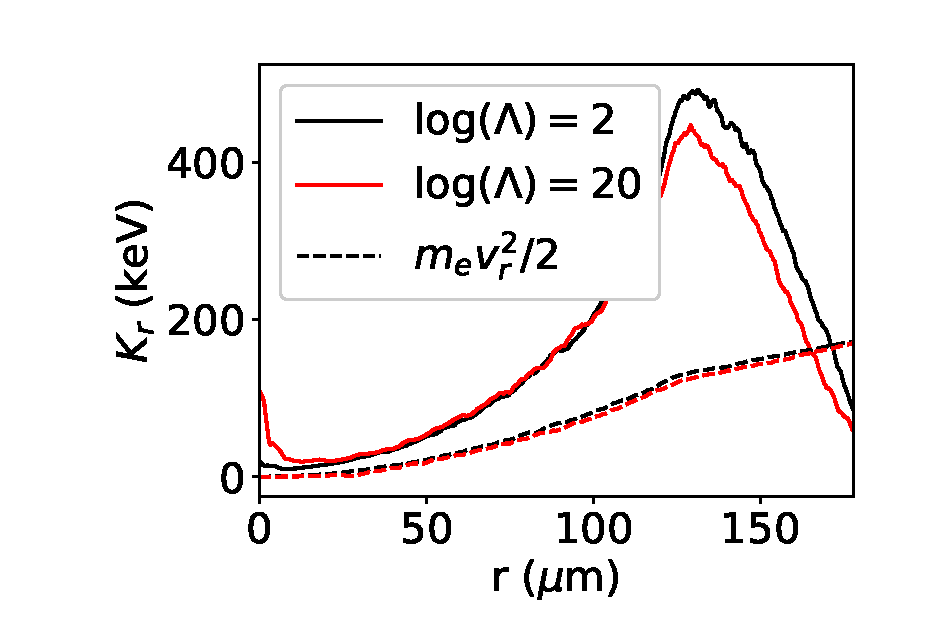
\includegraphics[width=0.33\textwidth]{Tr_MHD_sup.eps}\\
\end{tabular}}
\caption{\label{fig:nt} 
(a) Hot electron  density.
(b) Cold (energy smaller than $100$ eV) electrons density.
(c) Hot electron drift velocity extracted from the radial first momentum of the distribution function, $\langle p_r \rangle_h$ using, $v_r=\langle p_r \rangle_h / (1+\langle p_r \rangle_h^2)^{1/2}$.
(d,e,f) $x$-aligned, radial and poloidal momentum flux averaged over the hot electron population. 
The drift contribution to the radial momentum flux is superimposed on (f) as dashed lines.
All profiles are extracted from the  PIC-MHD simulation at $t=0.5$ ps with $T_{h0} = 1\,\mathrm{MeV}$, $T_{c0} = 50\,\mathrm{eV}$, $n_{h0} = 5 \times 10^{21}\, \mathrm{cm}^{-3}$ and $R_0 = 30\,\mu\mathrm{m}$ with $\log(\Lambda)=2$ (black) and $\log(\Lambda)=20$ (red).
}
\end{figure}
\begin{figure}[ht]
\centerline{\begin{tabular}{c}
%(a) $n_h(t)$ & (b) $T_c$ \\
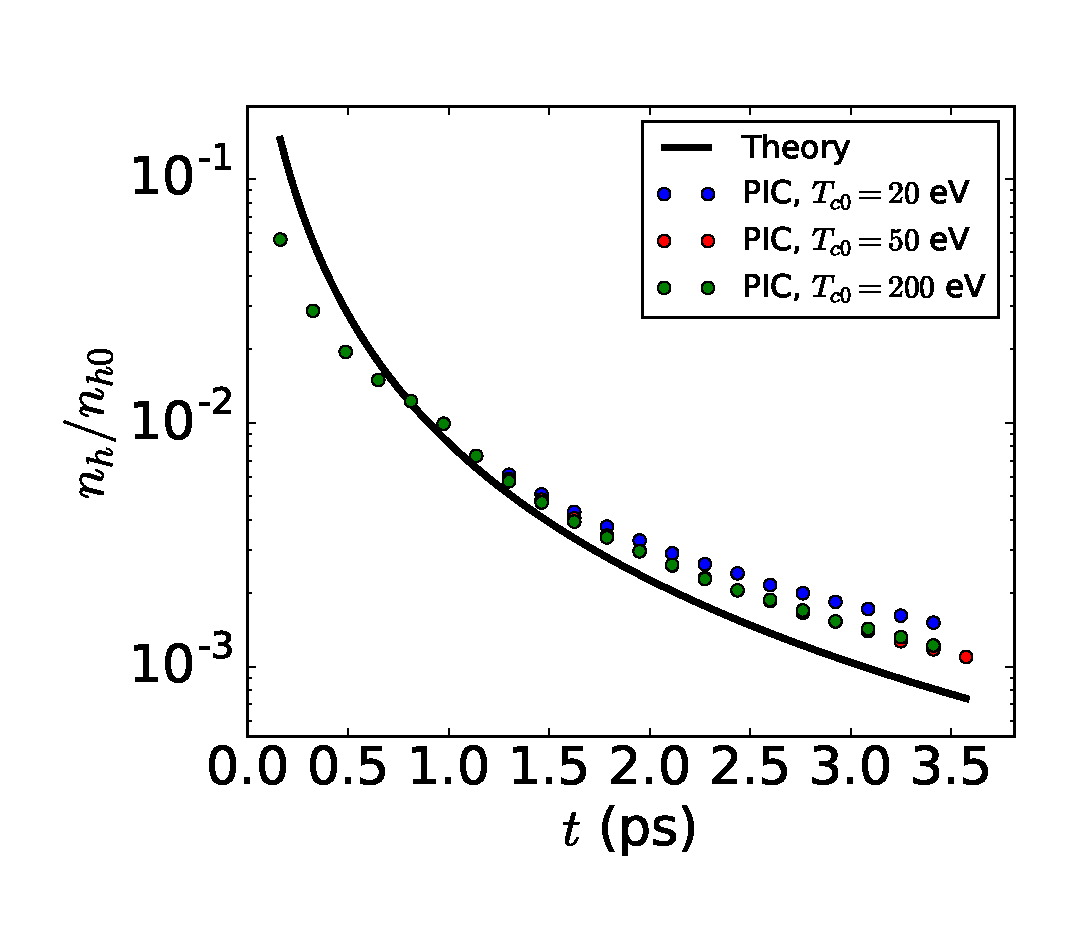
\includegraphics[width=0.33\textwidth]{nh_ne300_nh5_Th1MeV.eps}
%&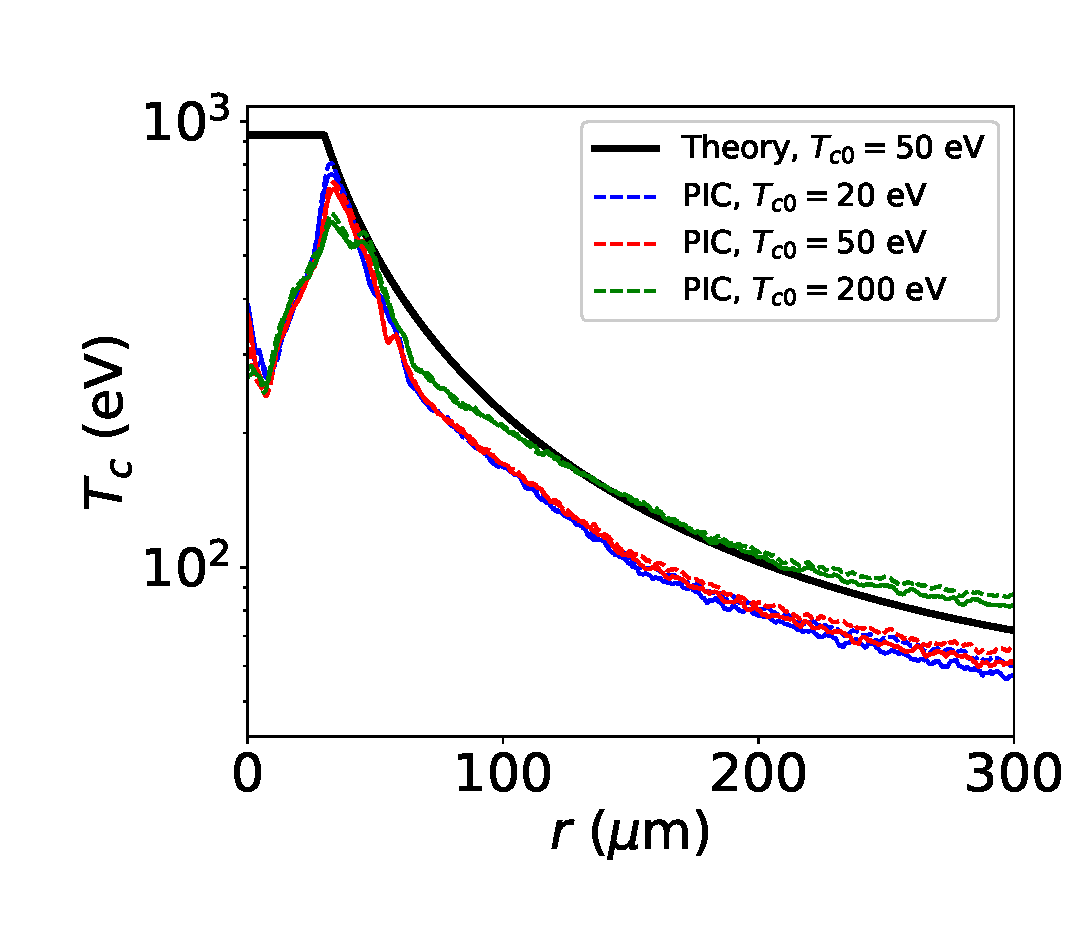
\includegraphics[width=0.33\textwidth]{Tec_ne300_nh5_Th1MeV.eps}
\end{tabular}}
\caption{\label{fig:n_param} 
Evolution as a function of time of the hot electron density averaged over $100\, \mu$m$<r<300\, \mu$m.
%(b) Cold electron temperature profile for $T_{c0}= 20$ eV (blue), $ 50$ eV (red) and $ 200$ eV (green)   at $t=2.6$ (dashed line) and $3.4$ ps  (plain line). 
The other parameters of the PIC MHD simulation are $n_{h0}=5\times 10^{21}$ cc, $T_{h0}=1 MeV$, $n_{c0} = 3\times 10^{23}$ cm$^{-3}$.
%The prediction of Eqs. \eqref{eq:tc}-\eqref{eq:tc2} for $T_{c0}= 50$ eV and $n=3/2$ and $n_c =  6\times 10^{23}\, \mathrm{cm}^{-3}$  is in plain black line.
}
\end{figure}

\section{ Sensitivity of the diagnostics to the Weibel instability in the expanding plasma} 

\subsection{Deflection of a probing proton off magnetic fluctuations}
The proton radiographs obtained experimentally presents small contrasts variations and are therefore not in the so-called caustics regime, implying that the probing protons were weakly deflected by the self-generated fields.
Reference \cite[]{RSI_protograhyb} proposes a  deflection angle estimates that can be applied to our study.
The case of cylindrical Gaussian current filament is addressed in Sec. VI.D., using a radial extent of $a\equiv\lambda_p$ and a longitudinal length given be the target thickness $b\equiv L_p$.

The numerical applications of  Sec. VI.D. of Ref. \cite[]{RSI_protograhyb} are presented in the limit of   elongated filaments ($b\equiv L_p\gg a\equiv\lambda_p $). In our case where the filament  extends on the thickness of the target, $L_p$  verifies $ L_p \lesssim \lambda_p$ and the resulting deflection angle is given by the combination of Eqs. (53), (54) and (102) for $d = ( \lambda_p^2\cos^2\theta + L_p^2 \sin^2 \theta)^{1/2} \simeq  \lambda_p$ (where $\theta$ is the probing angle of protons normal to the target that verify $\theta\lesssim 0.1$) and reads
\begin{equation}\label{eq:alphaphith}
\alpha^B_x(x_0,y_0) \simeq \pi^{1/2} x_0 \frac{L_p }{\lambda_p}  \frac{e B_p }{m_p v_p} \exp\left(-\frac{x_0^2}{\lambda_p^2}-\frac{y_0^2}{ \lambda_p^2} \right)\, ,
\end{equation}
where we introduced the position $x_0$ and $y_0$ of the probing proton relatively to the center of the current filament.
Maximizing the above equation relatively to $x_0$ and $y_0$ gives
\begin{equation}
\alpha^B_p = \max_{x_0,y_0}[\alpha_x(x_0,y_0) ] \simeq \frac{\pi^{1/2}}{2\exp(1/2)} \frac{e  B_p L_p }{m_p v_p}\, . \label{eq:alaphaphi}
\end{equation}
The resulting deflection angle thus depends on the magnetic field amplitude,  $  B_p$ at saturation and on the dominant wavelength of the probed Weibel instability.
The instability that results from the refluxing of electrons in the expanding plasma creates magnetic field typical wavelength \cite[]{PRL_Gode_2017} given by the electron skin depth of the hot electrons 
\begin{equation}\label{eq:lp}
\lambda_p \simeq 2\pi\gamma_h^{1/2} \frac{c}{\omega_{ph}} \, ,
\end{equation}
and of magnetic field amplitude given by 
\begin{equation}\label{eq:bp}
B_p \simeq \frac{m_e\omega_{ph}}{2\pi\gamma_h^{1/2} e}\, ,
\end{equation}
where $\gamma_h^{1/2}$ is the Lorentz factor of the hot electrons, close to unity in our case.
The length of the filament can be related to the scale length of the expanding underdense plasma, $L_p = c_{s} t$, where $c_{s}$ is the hot electron sound speed.
Applying the above estimates to the full 2D PIC simulation at $t = 1.44$ ps, gives for $D=\delta=1$, $n_h  \sim  8 \times 10^{19}$ cm$^{-3}$.
 and $\lambda_p \sim 4 \, \mu$m 
and  $B_p \sim 509$ T in good agreement with the lineout of Fig. \ref{fig:cut}(a) which gives  $\lambda_p \sim 6.6 \, \mu$m 
and  $B_p \sim 500$ T.

In the experiment $(D,\delta)=(2,1)$ at 4 ps, the hot electron density is $n_h\simeq 4.1\times 10^{17}$ cm$^{-3}$  [Eq. \eqref{eq:nt} for $n_{h0}=5\times 10^{21}$  cm$^{-3}$ and $R_0=30\, \mu$m], which gives $\lambda_p\simeq 52\, \mu$m and a magnetic field of approximately $\sim 33$ T. 
At this time, the length of the filament is around  $L_p \sim c_st \sim 38\, \mu$m, which is of the order of $\lambda_p$.
Hence, the maximum deflection angle resulting from  the magnetic filaments probed in the direction of the current derives from Eq. \eqref{eq:alaphaphi} replacing $\lambda_\phi$ and $B_\mathrm{sat}$ by $\lambda_p$ and $B_p$.

%%directly from Eq. (104) of \cite[]{RSI_protograhyb} and reads
\begin{equation}
\alpha^B_p \simeq  \frac{\pi^{1/2}}{2\exp(1/2)}      \frac{m_eL_p\omega_{ph}}{2\pi\gamma_h^{1/2}m_p v_p} \, . \label{eq:alaphap}
\end{equation}
Hence, the probing proton deflection angle $\alpha_p$ (and therefore the RCF dose variation) induced by the Weibel-induced magnetic field triggered in the expanding plasma should 
depend on the plasma parameters as $\omega_pL_p$. Using of $L_p \sim c_st $ and Eq. \eqref{eq:nt} for $(D,\delta)=(2,1)$, we obtain $\alpha^B_p\propto cs/(1+c_st/L)^{1/2}$ (for $t\gg R_0/c\simeq 100$ fs). The probing proton deflection angle should therefore slowly decreases as the   target expands and on hydrodynamical times scales.
This is in qualitative accordance with the experimental observation showing a weak temporal evolution of the proton dose variation over the 10s of picoseconds of the experimental observations.

\begin{figure}[ht]
\centerline{\begin{tabular}{cc}
%(a) $E_y$ (MV/m) & 
(a) $B_z$ & (b)  $E_y$   \\
%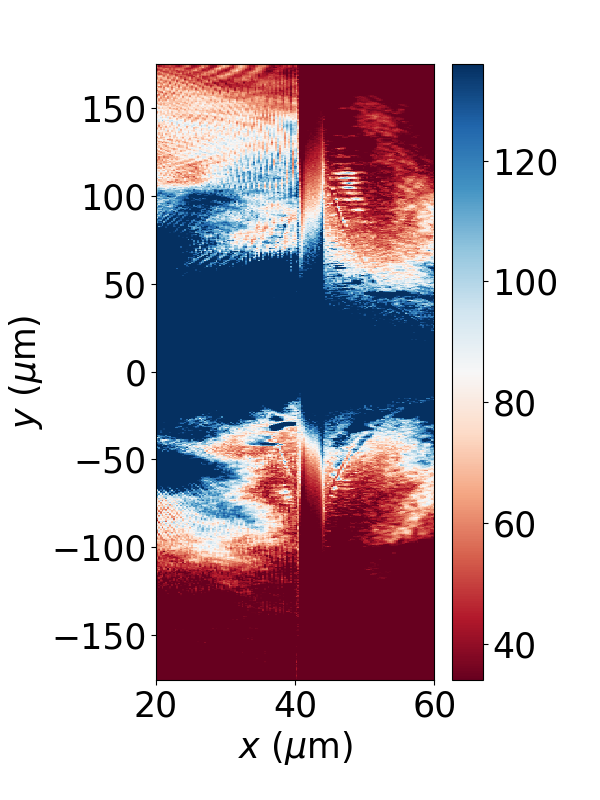
\includegraphics[scale=0.4]{Ey_t104000_nat.png}
%&
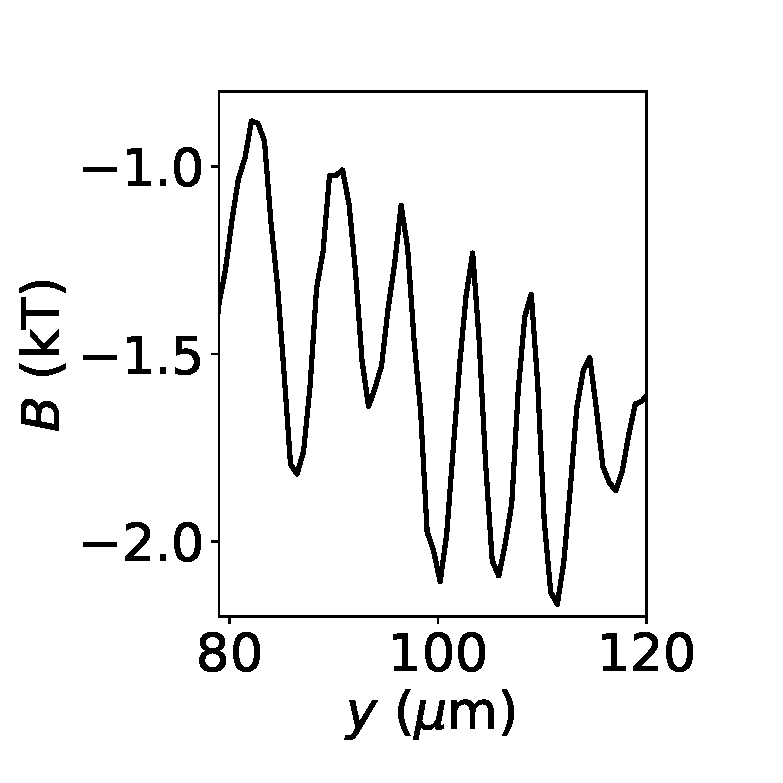
\includegraphics[scale=0.4]{Bzcut_t104000_nat.eps}
&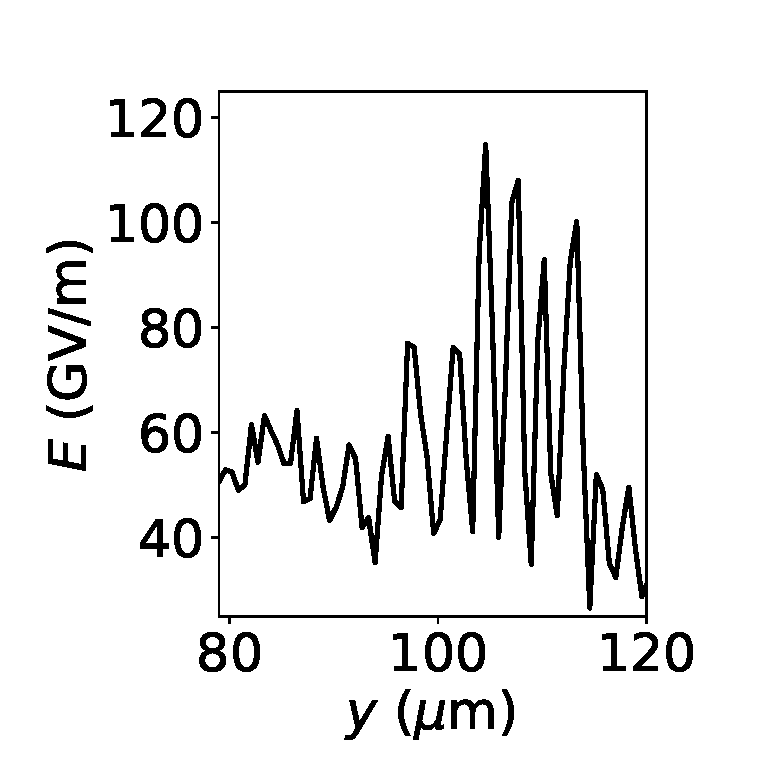
\includegraphics[scale=0.4]{Eycut_t104000_nat.eps}
\end{tabular}}
\caption{\label{fig:cut} 
%(a) $E_y$ component of the electric field in MV/m
Lineout at $x = 48\,\mu$mof   $B_z$ in kT (a) and $E_y$ in GV/m (b)  for the full PIC 2D simulation at $1.44$ ps.
}
\end{figure}

\subsection{Deflection of a probing proton off electric fluctuations}
 We address here the sensitivity of the probing protons to the electric field that develops around the current filaments in the expanding plasma.
Although, of mainly magnetic nature, the Weibel instability can trigger, in its saturated regime, electric fields  that may influence the proton radiographic measurements.
As pointed out in Refs. \cite{POP_Dieckmann_2009, POP_Bret_Gremillet_2010}, the current-carrying electrons  are,  unlike the ions,  pinched by the magnetic field loops . Hence, an electric field  results from the charge imbalance between the  ions and electrons which amplitude, in first approximation, may be estimated by a balance with the  magnetic pressure, $E_p \sim  - \nabla B_p^2/(2 \mu_0e n_h)$. 
Using Eqs. \eqref{eq:lp} and  \eqref{eq:bp}, we obtain  for $\nabla\equiv 2\pi/\lambda_p$
\begin{align}
E_p& \sim -  \frac{2\pi}{\lambda_p} \frac{B_p^2}{ \mu_0 e n_h }
\sim -  \frac{e\lambda_pB_p^2}{  2\pi  m_e } \, ,
 \label{eq:ep1}  \\
E_p& \sim\frac{m_ec\omega_{ph}}{4\pi^2\gamma_h^{3/2} e} \label{eq:ep}
 \, .
\end{align}
Note that such estimates has been used  in Refs. \cite{POP_Dieckmann_2009,POP_Ruyer_2015,PRL_Gode_2017} for comparison with experiments and numerical results.  
For our 2D full PIC simulation, we obtain $E_p\sim 24 $ GV/m which is fairly consistent with Fig. \ref{fig:cut}(b). Moreover, the  wavelength evidenced by our numerical results is roughly twice smaller for the electric modulations than for the magnetic ones, as predicted by Eq. \eqref{eq:ep}. Regarding the experiment, the electric field modulation amplitude verifies  $E_p \sim 1.5$ GV/m at $t=4$ ps.

As in Sec. IV.A, the typical probing proton deflection angle is obtained by combining Eq.  (53)-(55) of Ref. \cite[]{RSI_protograhyb} for $d\simeq a= \lambda_p/2 $
with $\theta \ll 1$. 
It is given by the ratio between the electric potential jump $\Phi_p\sim E_p(\lambda_p/2)/(2\pi)$ and the proton energy $W = m_pv_p^2/2$ 
\begin{equation}\label{eq:alphaep0}
\alpha^E_p \simeq \pi^{1/2}  \frac{L_p}{\lambda_p/2} \frac{e \Phi_p }{W}  \mathrm{max}_{x_0,y_0}\left[  
\frac{x_0}{\lambda_p/2}\exp\left(-\frac{x_0^2}{(\lambda_p/2)^2}-\frac{y_0^2}{ (\lambda_p/2)^2} \right) 
\right] \, .
\end{equation}
We thus obtain
\begin{equation}\label{eq:alphaep}
 \alpha^E_p \sim \frac{\pi^{1/2}}{2\exp(1/2)} \frac{L_p}{\lambda_p/2} \frac{e \Phi_p }{W} 
 %\sim \frac{\pi^{1/2}}{2\exp(1/2)}  \frac{L_p e E_p}{2\pi W}  
 \sim  \frac{\pi^{1/2}}{2\exp(1/2)}   \frac{m_ecL_p\omega_{ph}}{4\pi^3\gamma_h^{3/2}m_p v_p^2 }
 \, .
\end{equation}

Interestingly,  $\alpha^E_p$ presents the same dependence on the plasma parameters as  $\alpha^B_p$,  $\alpha^E_p\propto L_p \omega_{ph}$.  The ratio $\alpha^E_p/\alpha^B_p =c/(2\pi^2v_p)$  is typically $\sim 35-50$\% for our  probing proton energy (between $4$ and $9.5$ MeV), and therefore can affect  the experimental measurements.

\subsection{Influence of the electric and magnetic fields topology on the resulting radiographs}
Since this electric field tends to compensate the pinching magnetic force on the electron population, it is radial and points toward the center of each current filament in the expanding plasma. Such topology tends to focus the probing protons toward the center of the filament independently of the polarity of the current (induced by  the hot electrons or by the target return current ) or of the side of the target (front side or back side) in which the instability is triggered. 
It contrasts with the influence of the magnetic field on the probing protons which focusing or defocussing character depends on the polarity of the current and on the side of the target. Indeed,  in the back (respectively front) side of the target, the return current filaments are focusing (defocussing) whereas the   particles leaving the target  tends to induce a defocussing (focusing) magnetic loop [see Fig. 2(e) of the main paper].

Overall,   at least two sets of field structures  are to be considered, the magnetically focusing  and  defocussing ones which  results in black and white spots respectively. 
The electric field which is always focusing, partly  fade the white spots from the RCF and increase the contrast of the dark spots.  
Since the electric field profile has a quadratic dependence on the magnetic field, its influence on the radiographs is more and more significant over the $B$-field contribution as the amplitude of $B_\theta$  increases. Likewise,  the electric field amplitude is proportional to the magnetic wavelength [or inversely proportional to $n_e\lambda_p$, see Eq. \eqref{eq:ep1}] so that varying the 
parameters $a$ and $\lambda_p$ of Eqs. (6) and (7) of the main paper,
allows to evidence various structures that may arise in the radiographs depending on the field profiles.

\begin{figure}[ht]
\centerline{\begin{tabular}{ccc}
(a) $ \lambda_p =100\, \mu$m  & (b) $ \lambda_p =120\, \mu$m  & (c)  $ \lambda_p =200\, \mu$m   \\
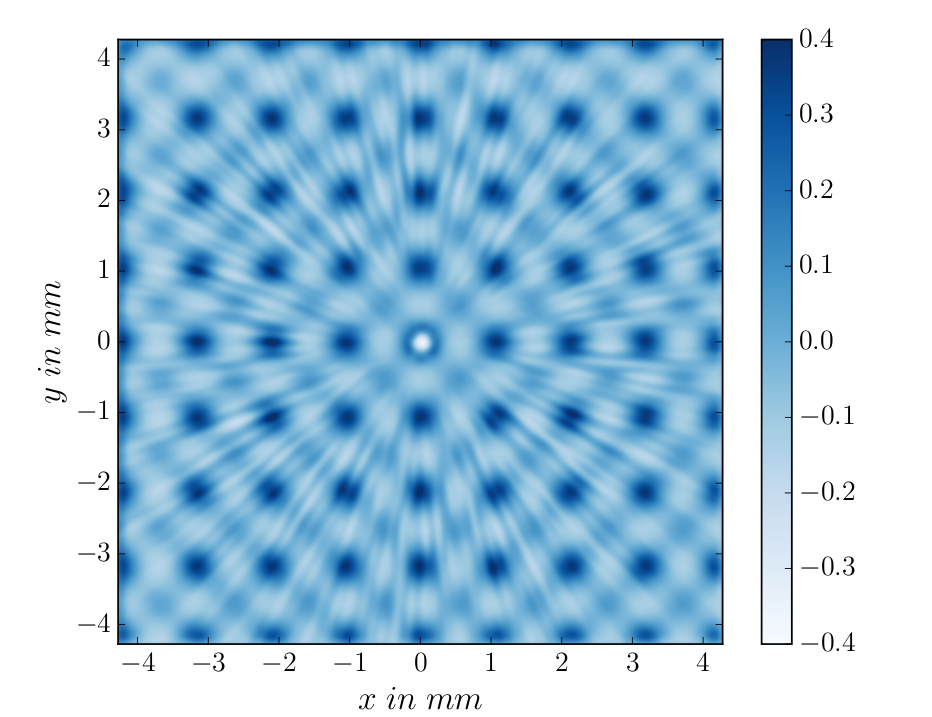
\includegraphics[scale=0.15]{p_radio_conv_2D5_Alu_10T_a60_l140.png}
&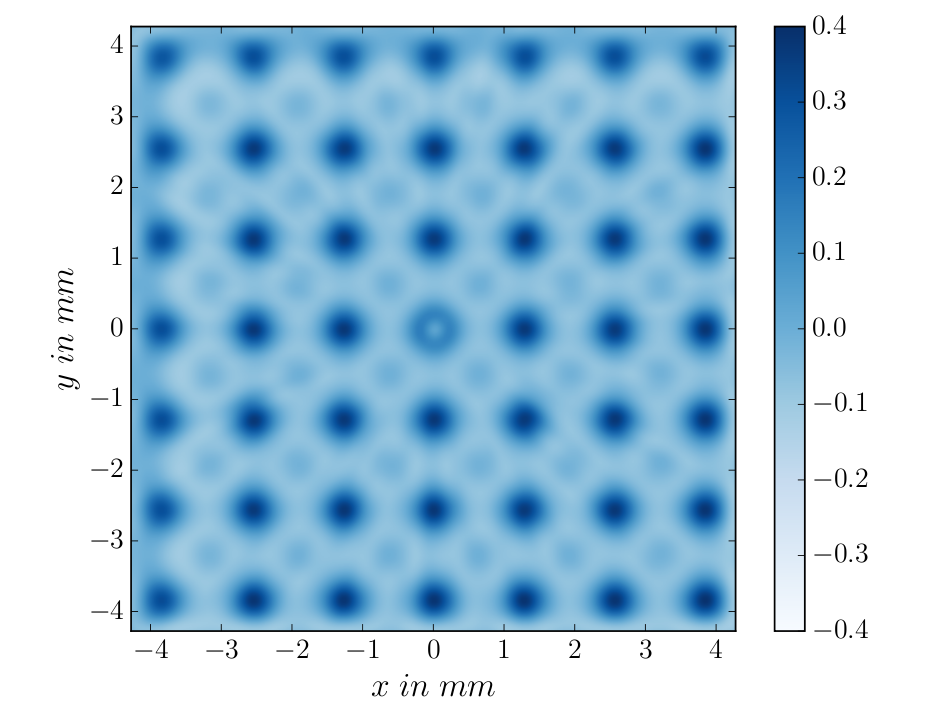
\includegraphics[scale=0.15]{p_radio_conv_2D5_Alu_10T_a60_l169.png}
&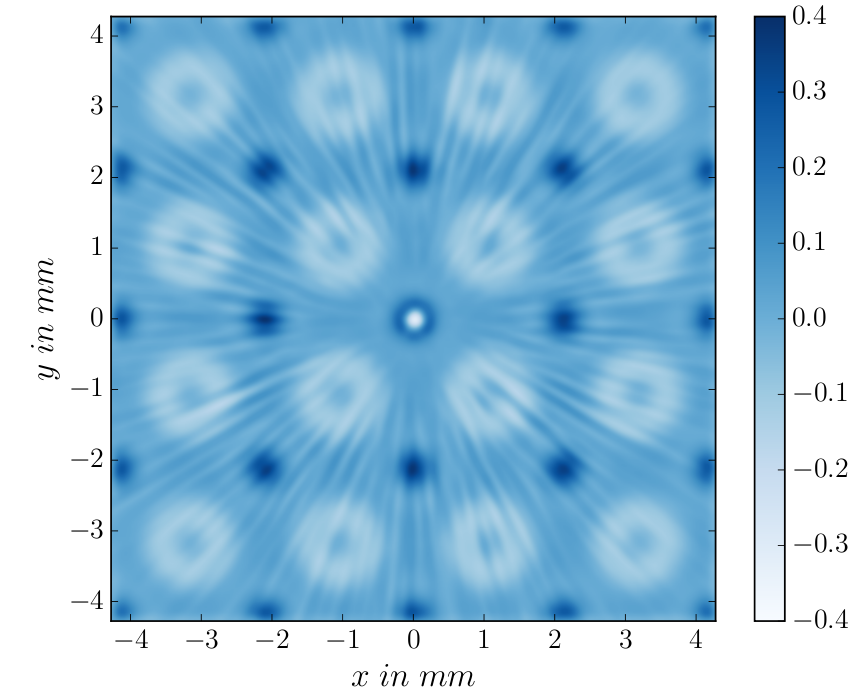
\includegraphics[scale=0.15]{p_radio_conv_2D5_Alu_10T_a60_l280.png}
\end{tabular}}
\caption{\label{fig:radiosup}  
%\textcolor{red}{verifier les parametres, refaire les figures (?)}
Modeled radiographs using the low resitivity PIC MHD simulation results  with superimposed filaments extending in the z direction.
The Lorentz force around the  filaments  are given by Eqs. (6) and (7) of the main paper with $L_p = 48 \, \mu$m, $B_0= 10$ T and $a = 60\, \mu$m, placed on one side of the target.
The minimum distance between each filament of same magnetic polarity is $ \lambda_p =100\, \mu$m  (a), $ \lambda_p =120\, \mu$m  (b) and $ \lambda_p =200\, \mu$m   (c).
All scales are on the detector plane.
}
\end{figure}
For  $ \lambda_p =100\, \mu$m [see Fig. \ref{fig:radiosup}(a)]  dark spots and dark lines  may be seen. As  $ \lambda_p$ increases from $120\, \mu$m  to   $ 200\, \mu$m, the dark lines disappear living only dark spots [see Fig. \ref{fig:radiosup}(b)], which, in turn, leave place to dark spot surrounded by white loops [see Fig. \ref{fig:radiosup}(c)]. Qualitatively similar structures can be seen in the simulated radiographs shown in Figs. 2(a,b,c) of the main paper at various times and positions. 
The radiographs at $t =20$ ps  [Fig. 2(c) of the main paper] presents more dark spots surrounded by white loops than at $t= 13.5$ ps  [Fig. 2(b)],  which, as suggested by Figs. \ref{fig:radiosup}(b,c), is qualitatively consistent with  an increase of the magnetic wavelength caused by the plasma expansion and therefore a decreasing electron density.

A few hundreds of microns away from the irradiated region, the target is likely to expand on the front and the rear side. 
For thin enough targets like in our case, one may expect both expansion to behave similarly, so that the  Weibel-induced electric and magnetic fields should develop with comparable wavelength and field amplitudes. 
In order to explore the contribution of both  sides of the target on the proton radiographs, we have performed ILZ simulations with two  sets of electromagnetic filaments shifted trans
To the best of our knowledge, no constrains on the relative position of the filaments on the two sides of the target can be found. 
Figures \ref{fig:radiosup2}(a) a case where the electric and magnetic fields of the two expanding region, separated by the three microns-thickness of the foil,  are shifted from half a magnetic wavelength on the $y$ direction. The horizontal lines that appears on the simulated RCF are the consequence of the focusing filaments that become aligned when projected on the detector.
Interestingly, when the field pattern are shifted by a full wavelength (so that the magnetic field loops are anti-aligned), like in  Fig. \ref{fig:radiosup2}(b),  dark points can be seen. In this case, the magnetic field contribution from both sides of the target cancel each other and the dominant deflecting field for the probing protons is the  electrostatic field that is always focusing.
 
\begin{figure}[ht]
\centerline{\begin{tabular}{cc}
(a) & (b)   \\
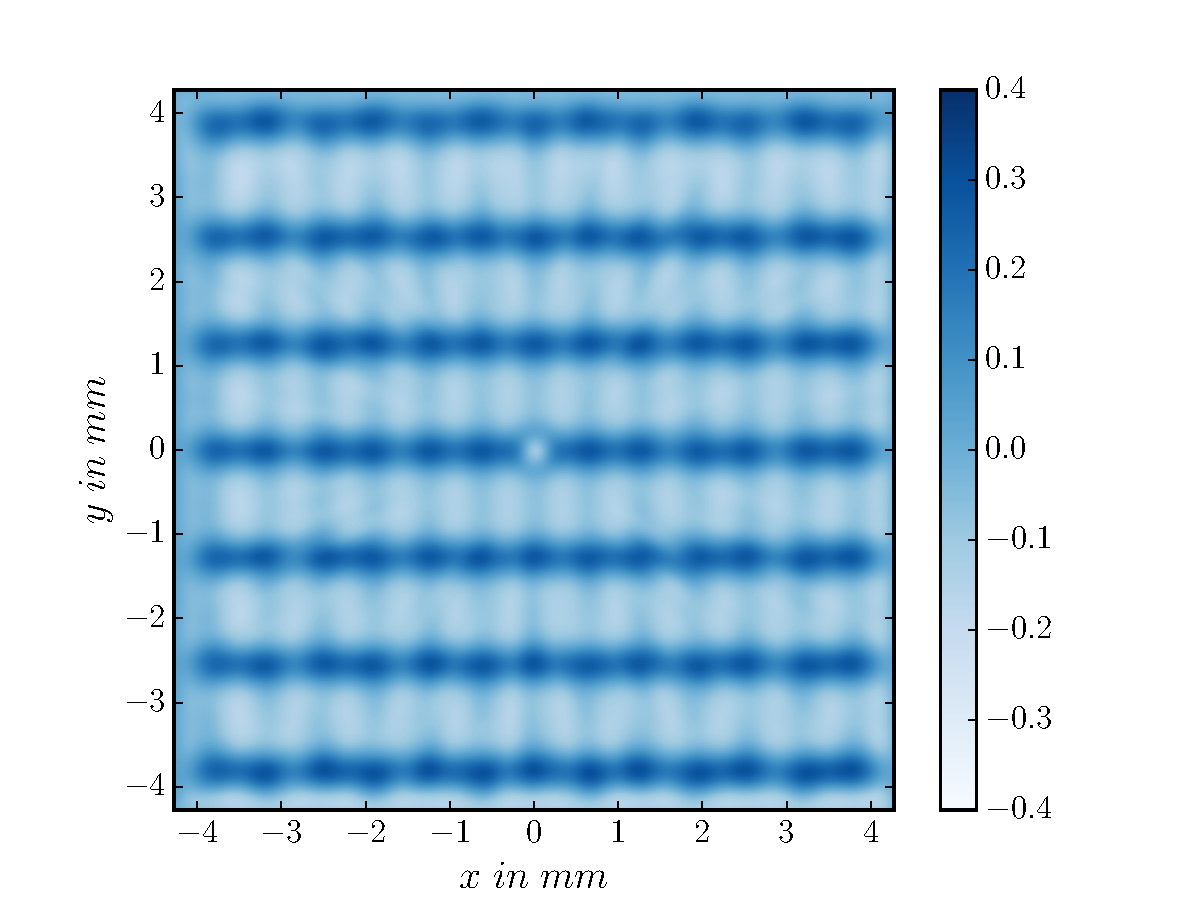
\includegraphics[scale=0.3]{p-radio_conv_2D5_Al_2sAntiF_10T_a60u_lb120u_vCR2.pdf}
%&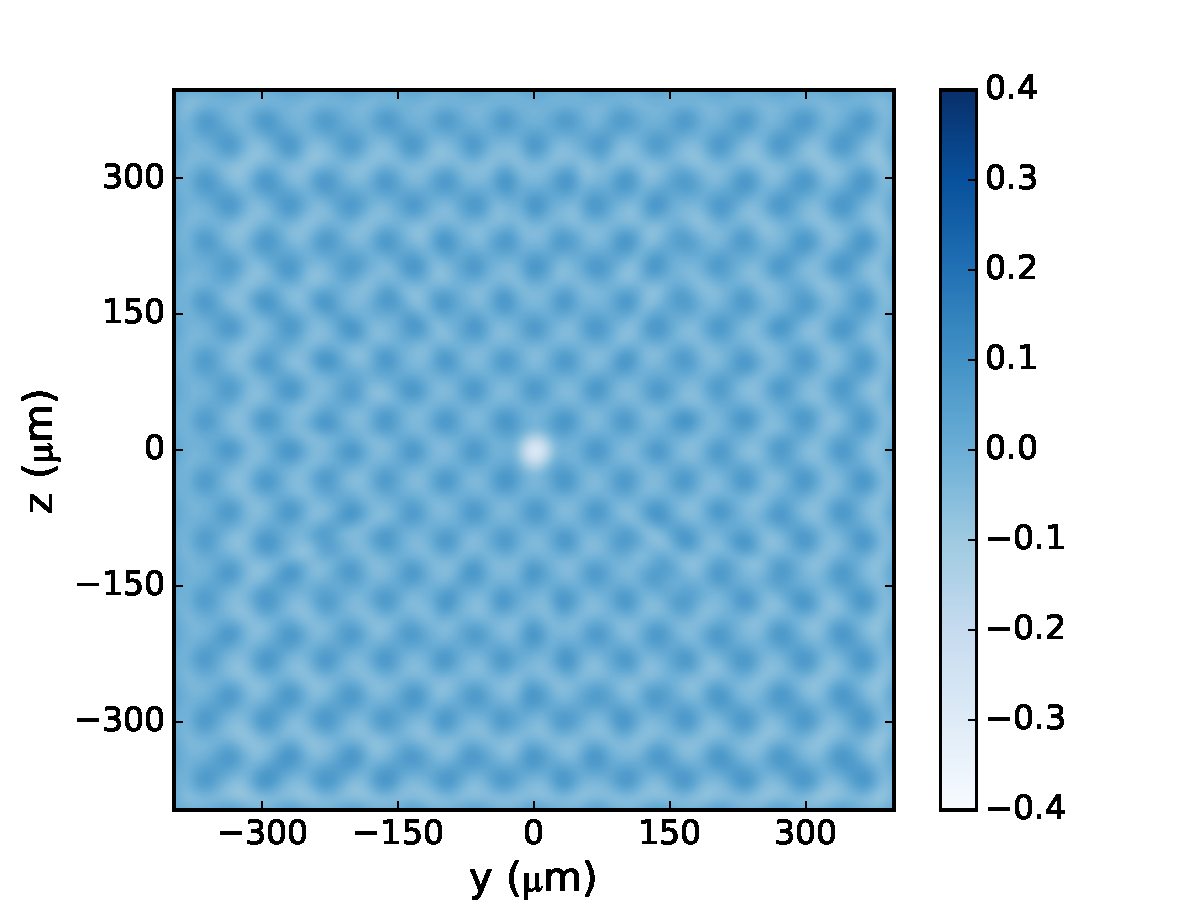
\includegraphics[scale=0.25]{p-radio_conv_2D5_Alu_2sPhase_7T_a34u_lb68u_vCR2.pdf} 
&\includegraphics[scale=0.3]{p-radio_conv_2D5_Alu_2sPhase_10T_a60u_lb120u_vCR2.pdf}
\end{tabular}}
\caption{\label{fig:radiosup2}  
%\textcolor{red}{verifier les parametres, refaire les figures (?)}
Modeled radiographs using the low resitivity PIC MHD simulation results  with superimposed filaments extending in the z direction.
The fields have the same parameters than in Fig. \ref{fig:rcf_supp}(b), with the contribution of both the rear and the front side of the target accounted for (see text).
The electric and magnetic field profiles have been shifted by half a wavelength for (a) and by a full wavelength in (b), so that the magnetic field loops are anti-aligned from one side of the target to the other.
}
\end{figure}

%\section{Alternative scenarios}
%Other possible scenarios which may explain these structures will be here ruled out. 
%\subsection{Weibel in dense part of the irradiated region}
%One simple explanation would be that the proton deflections are due to the well-known electron current-filamentation instability arising in the solid target close to the high-intensity focal spot \cite[]{PRL_Sentoku_2003}. The probing protons  would then be subject to the small-scale B-fields generated close to the laser-irradiated region before being deflected by the large-scale surface Biermann-Battery B-field.  
%However, the size of the measured loop structures ($\sim 100 \,\mu\mathrm{m}$) is not consistent with the typical scale of the involved $B$-field close to the dense plasma electron skin-depth $c/\omega_{pe}\simeq 0.5\,\mu$m where $\omega_{pe}=(n_e e^{2}/m_e\epsilon_0)^{1/2}$ is the electron plasma frequency ($n_e$, $m_e$ are the electron density and mass respectively; $e$ and $\epsilon_0$ are the electron charge and vacuum permittivity respectively).
%Here we used $n_e \simeq 180 \times 10^{21}\,\mathrm{cm}^{-3}$ for the electron density of the Al$^{3+}$ target ($Z*=3$ corresponds to the ionization state at moderate temperatures $\gtrsim 10\,\mathrm{eV}$). 
%In addition, the resolution of the diagnostic is limited by the proton source size of a few microns which prevents the detection of such small scale B-field structures  \cite[]{POP_Fuchs_2007}.  All this invalidates this first scenario.
%
%\subsection{Filamentation in the expanding plasma close to the focal spot}
%The typical length of the observed loops, much larger than the dense plasma electron-skin depth, may suggest another scenario where the instability takes place in the under-dense part of the expanding plasma on each side of the target, where the plasma skin-depth is much larger. However, the observed filaments are located several $100\,\mu\mathrm{m}$ away from  the irradiated area, where little expansion is expected to take place as was measured in a previous experiment at similar laser intensities \cite[]{PRL_Antici_2008}.
%Moreover, the proton radiographs evidence a planar and regular distribution of the observed structures, which contradicts a 3D spreading of the filaments in the under-dense plasma plume.
%
%\subsection{Weibel instability induced by the probing protons through the Al foil}
%The time spent by the probing protons through the Al foil, $\delta t \simeq 3 \, \mu\mathrm{m} / v_i  \lesssim 200\,\mathrm{fs}$ (for $\gtrsim 4\,\mathrm{MeV}$ protons), is more than an order of magnitude smaller than the typical growth time of the current filamentation instability between the probing protons and the Al target of $\Gamma^{-1}\simeq \omega_{pi}^{-1} c/v_i\gtrsim 5$ ps (for a proton density $\lesssim 10^{19}\,\mathrm{cm}^{-3}$). 
%Moreover, the radiographs obtained without irradiation of the Al foil do no present any proton deflections. Hence, the probing protons alone cannot trigger any electromagnetic instability while they cross the Al target.


\begin{thebibliography}{10}
\expandafter\ifx\csname url\endcsname\relax
  \def\url#1{\texttt{#1}}\fi
\expandafter\ifx\csname urlprefix\endcsname\relax\def\urlprefix{URL }\fi
\providecommand{\bibinfo}[2]{#2}
\providecommand{\eprint}[2][]{\url{#2}}

\bibitem{Shkarofsky_1966}
\bibinfo{author}{Shkarofsky, I.}, \bibinfo{author}{Johnston, T.} \&
  \bibinfo{author}{Bachynski, M.}
\newblock \emph{\bibinfo{title}{The Particle Kinetics of Plasmas}}
  (\bibinfo{publisher}{Addison-Wesley Pub. Co.}, \bibinfo{year}{1966}).

\bibitem{Belmont_2013}
\bibinfo{author}{{Belmont}, G.}, \bibinfo{author}{Roland, G.},
  \bibinfo{author}{Mottez, F.}, \bibinfo{author}{Pantellini, F.} \&
  \bibinfo{author}{Pelletier, G.}
\newblock \emph{\bibinfo{title}{{Collisionsless plasmas in astrophysics}}}
  (\bibinfo{publisher}{Wiley}, \bibinfo{year}{2013}).

\bibitem{Davidson_1983}
\bibinfo{author}{Davidson, R.~C.}
\newblock \bibinfo{title}{Kinetic waves and instabilities in uniform plasmas}.
\newblock In \bibinfo{editor}{Rosenbluth, M.~N.} \& \bibinfo{editor}{Galeev,
  R.~Z.} (eds.) \emph{\bibinfo{booktitle}{{Handbook of Plasma Physics}}},
  vol.~\bibinfo{volume}{1} (\bibinfo{publisher}{North-Holland},
  \bibinfo{address}{Amsterdam}, \bibinfo{year}{1983}).

\bibitem{PRL_Weibel_1959}
\bibinfo{author}{Weibel, E.~S.}
\newblock \bibinfo{title}{Spontaneous growing transverse waves in a plasma due
  to an anisotropic velocity distribution}.
\newblock \emph{\bibinfo{journal}{Phys. Rev. Lett.}}
  \textbf{\bibinfo{volume}{2}}, \bibinfo{pages}{83--84} (\bibinfo{year}{1959}).

\bibitem{POF_Fried_1959}
\bibinfo{author}{Fried, B.~D.}
\newblock \bibinfo{title}{Mechanism for instability of transverse plasma
  waves}.
\newblock \emph{\bibinfo{journal}{Phys. Fluids}} \textbf{\bibinfo{volume}{2}},
  \bibinfo{pages}{337--337} (\bibinfo{year}{1959}).

\bibitem{POF_Davidson_1972}
\bibinfo{author}{Davidson, R.~C.}, \bibinfo{author}{Hammer, D.~A.},
  \bibinfo{author}{Haber, I.} \& \bibinfo{author}{Wagner, C.~E.}
\newblock \bibinfo{title}{Nonlinear development of electromagnetic
  instabilities in anisotropic plasmas}.
\newblock \emph{\bibinfo{journal}{Phys. Fluids}} \textbf{\bibinfo{volume}{15}},
  \bibinfo{pages}{317} (\bibinfo{year}{1972}).

\bibitem{PRL_Lee_1973}
\bibinfo{author}{{Lee}, R.} \& \bibinfo{author}{{Lampe}, M.}
\newblock \bibinfo{title}{{Electromagnetic Instabilities, Filamentation, and
  Focusing of Relativistic Electron Beams}}.
\newblock \emph{\bibinfo{journal}{Phys. Rev. Lett.}}
  \textbf{\bibinfo{volume}{31}}, \bibinfo{pages}{1390--1393}
  (\bibinfo{year}{1973}).

\bibitem{APJ_Jaroschek_2004}
\bibinfo{author}{{Jaroschek}, C.~H.}, \bibinfo{author}{{Lesch}, H.} \&
  \bibinfo{author}{{Treumann}, R.~A.}
\newblock \bibinfo{title}{{Self-consistent Diffusive Lifetimes of Weibel
  Magnetic Fields in Gamma-Ray Bursts}}.
\newblock \emph{\bibinfo{journal}{Astrophys. J.}}
  \textbf{\bibinfo{volume}{616}}, \bibinfo{pages}{1065--1071}
  (\bibinfo{year}{2004}).

\bibitem{PRL_Adam_2006}
\bibinfo{author}{Adam, J.~C.}, \bibinfo{author}{H\'{e}ron, A.} \&
  \bibinfo{author}{Laval, G.}
\newblock \bibinfo{title}{Dispersion and transport of energetic particles due
  to the interaction of intense laser pulses with overdense plasmas}.
\newblock \emph{\bibinfo{journal}{Phys. Rev. Lett.}}
  \textbf{\bibinfo{volume}{97}}, \bibinfo{pages}{205006}
  (\bibinfo{year}{2006}).

\bibitem{RPP_Marcowith_2016}
\bibinfo{author}{{Marcowith}, A.} \emph{et~al.}
\newblock \bibinfo{title}{{The microphysics of collisionless shock waves}}.
\newblock \emph{\bibinfo{journal}{Rept. Prog. Phys.}}
  \textbf{\bibinfo{volume}{79}}, \bibinfo{pages}{046901}
  (\bibinfo{year}{2016}).

\bibitem{APJ_Schlickeiser_2003}
\bibinfo{author}{{Schlickeiser}, R.} \& \bibinfo{author}{{Shukla}, P.~K.}
\newblock \bibinfo{title}{{Cosmological Magnetic Field Generation by the Weibel
  Instability}}.
\newblock \emph{\bibinfo{journal}{Astrophys. J. Lett.}}
  \textbf{\bibinfo{volume}{599}}, \bibinfo{pages}{L57--L60}
  (\bibinfo{year}{2003}).

\bibitem{PRL_Allen_2012}
\bibinfo{author}{Allen, B.} \emph{et~al.}
\newblock \bibinfo{title}{Experimental study of current filamentation
  instability}.
\newblock \emph{\bibinfo{journal}{Phys. Rev. Lett.}}
  \textbf{\bibinfo{volume}{109}}, \bibinfo{pages}{185007}
  (\bibinfo{year}{2012}).

\bibitem{PRL_Fox_2013}
\bibinfo{author}{Fox, W.} \emph{et~al.}
\newblock \bibinfo{title}{Filamentation instability of counter-streaming
  laser-driven plasmas}.
\newblock \emph{\bibinfo{journal}{Phys. Rev. Lett.}}
  \textbf{\bibinfo{volume}{111}}, \bibinfo{pages}{225002}
  (\bibinfo{year}{2013}).

\bibitem{NP_Huntington_2015}
\bibinfo{author}{Huntington, C.~M.} \emph{et~al.}
\newblock \bibinfo{title}{Observation of magnetic field generation via the
  weibel instability in interpenetrating plasma flows}.
\newblock \emph{\bibinfo{journal}{Nat. Phys.}} \textbf{\bibinfo{volume}{11}},
  \bibinfo{pages}{173--176} (\bibinfo{year}{2015}).

\bibitem{PNAS_Mondal_2012}
\bibinfo{author}{Mondal, S.} \emph{et~al.}
\newblock \bibinfo{title}{Direct observation of turbulent magnetic fields in
  hot, dense laser produced plasmas}.
\newblock \emph{\bibinfo{journal}{Proceedings of the National Academy of
  Sciences}} \textbf{\bibinfo{volume}{109}}, \bibinfo{pages}{8011--8015}
  (\bibinfo{year}{2012}).

\bibitem{POP_Gremillet_2002}
\bibinfo{author}{Gremillet, L.}, \bibinfo{author}{Bonnaud, G.} \&
  \bibinfo{author}{Amiranoff, F.}
\newblock \bibinfo{title}{Filamented transport of laser-generated relativistic
  electrons penetrating a solid target}.
\newblock \emph{\bibinfo{journal}{Phys. Plasmas}} \textbf{\bibinfo{volume}{9}},
  \bibinfo{pages}{941} (\bibinfo{year}{2002}).

\bibitem{JPP_Fiore_2010}
\bibinfo{author}{Fiore, M.}, \bibinfo{author}{Fiuza, F.},
  \bibinfo{author}{Marti, M.}, \bibinfo{author}{Fonseca, R.~A.} \&
  \bibinfo{author}{Silva, L.~O.}
\newblock \bibinfo{title}{Relativistic effects on the
  collisionless collisional transition of the filamentation instability in
  fast ignition}.
\newblock \emph{\bibinfo{journal}{J. Plasma Phys.}}
  \textbf{\bibinfo{volume}{76}}, \bibinfo{pages}{813­832}
  (\bibinfo{year}{2010}).

\bibitem{POP_Yang_2016}
\bibinfo{author}{Yang, X.~H.} \emph{et~al.}
\newblock \bibinfo{title}{Effects of filamentation instability on the
  divergence of relativistic electrons driven by ultraintense laser pulses}.
\newblock \emph{\bibinfo{journal}{Phys. Plasmas}}
  \textbf{\bibinfo{volume}{23}}, \bibinfo{pages}{103110}
  (\bibinfo{year}{2016}).

\bibitem{PRL_Fuchs_2003}
\bibinfo{author}{Fuchs, J.} \emph{et~al.}
\newblock \bibinfo{title}{Spatial uniformity of laser-accelerated
  ultrahigh-current mev electron propagation in metals and insulators}.
\newblock \emph{\bibinfo{journal}{Phys. Rev. Lett.}}
  \textbf{\bibinfo{volume}{91}}, \bibinfo{pages}{255002}
  (\bibinfo{year}{2003}).

\bibitem{PRL_MacLellan_2013}
\bibinfo{author}{MacLellan, D.~A.} \emph{et~al.}
\newblock \bibinfo{title}{Annular fast electron transport in silicon arising
  from low-temperature resistivity}.
\newblock \emph{\bibinfo{journal}{Phys. Rev. Lett.}}
  \textbf{\bibinfo{volume}{111}}, \bibinfo{pages}{095001}
  (\bibinfo{year}{2013}).

\bibitem{PRL_Storm_2009}
\bibinfo{author}{{Storm}, M.} \emph{et~al.}
\newblock \bibinfo{title}{{High-Current, Relativistic Electron-Beam Transport
  in Metals and the Role of Magnetic Collimation}}.
\newblock \emph{\bibinfo{journal}{Phys. Rev. Lett.}}
  \textbf{\bibinfo{volume}{102}}, \bibinfo{pages}{235004}
  (\bibinfo{year}{2009}).

\bibitem{PRE_Wei_2004}
\bibinfo{author}{{Wei}, M.~S.} \emph{et~al.}
\newblock \bibinfo{title}{{Observations of the filamentation of high-intensity
  laser-produced electron beams}}.
\newblock \emph{\bibinfo{journal}{Phys. Rev. E}} \textbf{\bibinfo{volume}{70}},
  \bibinfo{pages}{056412} (\bibinfo{year}{2004}).

\bibitem{PRL_Quinn_2012}
\bibinfo{author}{Quinn, K.} \emph{et~al.}
\newblock \bibinfo{title}{{Weibel}-induced filamentation during an ultrafast
  laser-driven plasma expansion}.
\newblock \emph{\bibinfo{journal}{Phys. Rev. Lett.}}
  \textbf{\bibinfo{volume}{108}}, \bibinfo{pages}{135001}
  (\bibinfo{year}{2012}).

\bibitem{PRL_Gode_2017}
\bibinfo{author}{G\"ode, S.} \emph{et~al.}
\newblock \bibinfo{title}{Relativistic electron streaming instabilities
  modulate proton beams accelerated in laser-plasma interactions}.
\newblock \emph{\bibinfo{journal}{Phys. Rev. Lett.}}
  \textbf{\bibinfo{volume}{118}}, \bibinfo{pages}{194801}
  (\bibinfo{year}{2017}).

\bibitem{NJP_Scott_2017}
\bibinfo{author}{Scott, G.~G.} \emph{et~al.}
\newblock \bibinfo{title}{Diagnosis of weibel instability evolution in the rear
  surface density scale lengths of laser solid interactions via proton
  acceleration}.
\newblock \emph{\bibinfo{journal}{New J. Phys.}} \textbf{\bibinfo{volume}{19}},
  \bibinfo{pages}{043010} (\bibinfo{year}{2017}).

\bibitem{POP_Heron_2015}
\bibinfo{author}{H\'eron, A.} \& \bibinfo{author}{Adam, J.~C.}
\newblock \bibinfo{title}{Physics of the interaction of ultra intense laser
  pulses with cold collisional plasma using large scale kinetic simulations}.
\newblock \emph{\bibinfo{journal}{Phys. Plasmas}}
  \textbf{\bibinfo{volume}{22}}, \bibinfo{pages}{072306}
  (\bibinfo{year}{2015}).

\bibitem{RSI_Albertazzi_2015}
\bibinfo{author}{Albertazzi, B.} \emph{et~al.}
\newblock \bibinfo{title}{A compact broadband ion beam focusing device based on
  laser-driven megagauss thermoelectric magnetic fields}.
\newblock \emph{\bibinfo{journal}{Rev. Sci. Instrum.}}
  \textbf{\bibinfo{volume}{86}} (\bibinfo{year}{2015}).

\bibitem{NF_Lefebvre_2003}
\bibinfo{author}{Lefebvre, E.} \emph{et~al.}
\newblock \bibinfo{title}{Electron and photon production from relativistic
  laser-plasma interactions}.
\newblock \emph{\bibinfo{journal}{Nucl. Fusion}} \textbf{\bibinfo{volume}{43}},
  \bibinfo{pages}{629--633} (\bibinfo{year}{2003}).

\bibitem{POP_Ren_2006}
\bibinfo{author}{Ren, C.} \emph{et~al.}
\newblock \bibinfo{title}{A global simulation for laser-driven {MeV} electrons
  in 50-$\mu$m {Fast Ignition} targets}.
\newblock \emph{\bibinfo{journal}{Phys. Plasmas}}
  \textbf{\bibinfo{volume}{13}}, \bibinfo{pages}{056308}
  (\bibinfo{year}{2006}).

\bibitem{POP_Dieckmann_2009}
\bibinfo{author}{Dieckmann, M.~E.}, \bibinfo{author}{Kourakis, I.},
  \bibinfo{author}{Borghesi, M.} \& \bibinfo{author}{Rowlands, G.}
\newblock \bibinfo{title}{One-dimensional particle simulation of the
  filamentation instability: Electrostatic field driven by the magnetic
  pressure gradient force}.
\newblock \emph{\bibinfo{journal}{Phys. Plasmas}} \textbf{\bibinfo{volume}{16}}
  (\bibinfo{year}{2009}).

\bibitem{POP_Bret_Gremillet_2010}
\bibinfo{author}{Bret, A.}, \bibinfo{author}{Gremillet, L.} \&
  \bibinfo{author}{Dieckmann, M.~E.}
\newblock \bibinfo{title}{Multidimensional electron beam-plasma instabilities
  in the relativistic regime}.
\newblock \emph{\bibinfo{journal}{Phys. Plasmas}}
  \textbf{\bibinfo{volume}{17}}, \bibinfo{pages}{120501}
  (\bibinfo{year}{2010}).

\bibitem{POP_Perez_2012}
\bibinfo{author}{{P\'erez}, F.}, \bibinfo{author}{{Gremillet}, L.},
  \bibinfo{author}{Decoster, A.}, \bibinfo{author}{Drouin, M.} \&
  \bibinfo{author}{Lefebvre, E.}
\newblock \bibinfo{title}{Improved modeling of relativistic collisions and
  collisional ionization in particle-in-cell codes}.
\newblock \emph{\bibinfo{journal}{Phys. Plasmas}}
  \textbf{\bibinfo{volume}{19}}, \bibinfo{pages}{083104}
  (\bibinfo{year}{2012}).

\bibitem{PRE_Mora_2005}
\bibinfo{author}{Mora, P.}
\newblock \bibinfo{title}{Thin-foil expansion into a vacuum}.
\newblock \emph{\bibinfo{journal}{Phys. Rev. E}} \textbf{\bibinfo{volume}{72}},
  \bibinfo{pages}{056401} (\bibinfo{year}{2005}).

\bibitem{PRL_McKenna_2011}
\bibinfo{author}{McKenna, P.} \emph{et~al.}
\newblock \bibinfo{title}{Effect of lattice structure on energetic electron
  transport in solids irradiated by ultraintense laser pulses}.
\newblock \emph{\bibinfo{journal}{Phys. Rev. Lett.}}
  \textbf{\bibinfo{volume}{106}}, \bibinfo{pages}{185004}
  (\bibinfo{year}{2011}).

\bibitem{PRE_Doumy_2004}
\bibinfo{author}{Doumy, G.} \emph{et~al.}
\newblock \bibinfo{title}{Complete characterization of a plasma mirror for the
  production of high-contrast ultraintense laser pulses}.
\newblock \emph{\bibinfo{journal}{Phys. Rev. E}} \textbf{\bibinfo{volume}{69}},
  \bibinfo{pages}{026402} (\bibinfo{year}{2004}).

\bibitem{PRL_Sarri_2012}
\bibinfo{author}{Sarri, G.} \emph{et~al.}
\newblock \bibinfo{title}{Dynamics of self-generated, large amplitude magnetic
  fields following high-intensity laser matter interaction}.
\newblock \emph{\bibinfo{journal}{Phys. Rev. Lett.}}
  \textbf{\bibinfo{volume}{109}}, \bibinfo{pages}{205002}
  (\bibinfo{year}{2012}).

\bibitem{PRL_Brunel_1987}
\bibinfo{author}{Brunel, F.}
\newblock \bibinfo{title}{Not-so-resonant, resonant absorption}.
\newblock \emph{\bibinfo{journal}{Phys. Rev. Lett.}}
  \textbf{\bibinfo{volume}{59}}, \bibinfo{pages}{52--55}
  (\bibinfo{year}{1987}).

\bibitem{PRL_Ping_2008}
\bibinfo{author}{Ping, Y.} \emph{et~al.}
\newblock \bibinfo{title}{Absorption of short laser pulses on solid targets in
  the ultrarelativistic regime}.
\newblock \emph{\bibinfo{journal}{Phys. Rev. Lett.}}
  \textbf{\bibinfo{volume}{100}}, \bibinfo{pages}{085004}
  (\bibinfo{year}{2008}).

\bibitem{CPC_Sokolov_2013}
\bibinfo{author}{Sokolov, I.~V.}
\newblock \bibinfo{title}{Alternating-order interpolation in a
  charge-conserving scheme for particle-in-cell simulations}.
\newblock \emph{\bibinfo{journal}{Computer Physics Communications}}
  \textbf{\bibinfo{volume}{184}}, \bibinfo{pages}{320 -- 328}
  (\bibinfo{year}{2013}).

\bibitem{PRSTAB_Lehe_2013}
\bibinfo{author}{Lehe, R.}, \bibinfo{author}{Lifschitz, A.},
  \bibinfo{author}{Thaury, C.}, \bibinfo{author}{Malka, V.} \&
  \bibinfo{author}{Davoine, X.}
\newblock \bibinfo{title}{Numerical growth of emittance in simulations of
  laser-wakefield acceleration}.
\newblock \emph{\bibinfo{journal}{Phys. Rev. ST Accel. Beams}}
  \textbf{\bibinfo{volume}{16}}, \bibinfo{pages}{021301}
  (\bibinfo{year}{2013}).

\bibitem{JCP_Vay_2011}
\bibinfo{author}{{Vay}, J.-L.}, \bibinfo{author}{{Geddes}, C.~G.~R.},
  \bibinfo{author}{{Cormier-Michel}, E.} \& \bibinfo{author}{{Grote}, D.~P.}
\newblock \bibinfo{title}{{Numerical methods for instability mitigation in the
  modeling of laser wakefield accelerators in a Lorentz-boosted frame}}.
\newblock \emph{\bibinfo{journal}{J. Comp. Phys.}}
  \textbf{\bibinfo{volume}{230}}, \bibinfo{pages}{5908--5929}
  (\bibinfo{year}{2011}).

\bibitem{JCP_Friedman_1990}
\bibinfo{author}{Friedman, A.}
\newblock \bibinfo{title}{A 2nd-order implicit particle mover with adjustable
  damping}.
\newblock \emph{\bibinfo{journal}{J. Comp. Phys.}}
  \textbf{\bibinfo{volume}{90}}, \bibinfo{pages}{292--312}
  (\bibinfo{year}{1990}).

\bibitem{JCP_Cohen_2010}
\bibinfo{author}{Cohen, B.}, \bibinfo{author}{Kemp, A.} \&
  \bibinfo{author}{Divol, L.}
\newblock \bibinfo{title}{Simulation of laser-plasma interactions and
  fast-electron transport in inhomogeneous plasma}.
\newblock \emph{\bibinfo{journal}{Journal of Computational Physics}}
  \textbf{\bibinfo{volume}{229}}, \bibinfo{pages}{4591 -- 4612}
  (\bibinfo{year}{2010}).

\bibitem{PRE_Stephens_2004}
\bibinfo{author}{Stephens, R.~B.} \emph{et~al.}
\newblock \bibinfo{title}{${K}_{\ensuremath{\alpha}}$ fluorescence measurement
  of relativistic electron transport in the context of fast ignition}.
\newblock \emph{\bibinfo{journal}{Phys. Rev. E}} \textbf{\bibinfo{volume}{69}},
  \bibinfo{pages}{066414} (\bibinfo{year}{2004}).

\bibitem{Decoster_1998}
\bibinfo{author}{Decoster, A.}, \bibinfo{author}{Markowich, P.},
  \bibinfo{author}{Perthame, B.} \& \bibinfo{author}{Raviart, P.}
\newblock \emph{\bibinfo{title}{Modeling of collisions}}.
\newblock Series in applied mathematics (\bibinfo{publisher}{Gauthier-Villars},
  \bibinfo{year}{1998}).

\bibitem{PRL_Cowan_2004}
\bibinfo{author}{Cowan, T.~E.} \emph{et~al.}
\newblock \bibinfo{title}{Ultralow emittance, multi-mev proton beams from a
  laser virtual-cathode plasma accelerator}.
\newblock \emph{\bibinfo{journal}{Phys. Rev. Lett.}}
  \textbf{\bibinfo{volume}{92}}, \bibinfo{pages}{204801}
  (\bibinfo{year}{2004}).

\bibitem{NIM_Highland_1975}
\bibinfo{author}{Highland, V.~L.}
\newblock \bibinfo{title}{Some practical remarks on multiple scattering}.
\newblock \emph{\bibinfo{journal}{Nuclear Instruments and Methods}}
  \textbf{\bibinfo{volume}{129}}, \bibinfo{pages}{497 -- 499}
  (\bibinfo{year}{1975}).

\bibitem{EPJ_Groom_2000}
\bibinfo{author}{Groom, D.~E.} \& \bibinfo{author}{Klein, S.~R.}
\newblock \emph{\bibinfo{journal}{Eur. Phys. J. C}}
  \textbf{\bibinfo{volume}{15}}, \bibinfo{pages}{163} (\bibinfo{year}{2000}).

\bibitem{RSI_Chen_2016}
\bibinfo{author}{Chen, S.~N.} \emph{et~al.}
\newblock \bibinfo{title}{Absolute dosimetric characterization of gafchromic
  ebt3 and hdv2 films using commercial flat-bed scanners and evaluation of the
  scanner response function variability}.
\newblock \emph{\bibinfo{journal}{Review of Scientific Instruments}}
  \textbf{\bibinfo{volume}{87}}, \bibinfo{pages}{073301}
  (\bibinfo{year}{2016}).

\bibitem{POP_Ruyer_2015}
\bibinfo{author}{Ruyer, C.}, \bibinfo{author}{Gremillet, L.},
  \bibinfo{author}{Debayle, A.} \& \bibinfo{author}{Bonnaud, G.}
\newblock \bibinfo{title}{Nonlinear dynamics of the ion weibel-filamentation
  instability: An analytical model for the evolution of the plasma and spectral
  properties}.
\newblock \emph{\bibinfo{journal}{Physics of Plasmas}}
  \textbf{\bibinfo{volume}{22}} (\bibinfo{year}{2015}).

\bibitem{RSI_protograhyb}
\bibinfo{author}{Kugland, N.~L.}, \bibinfo{author}{Ryutov, D.~D.},
  \bibinfo{author}{Plechaty, C.}, \bibinfo{author}{Ross, J.~S.} \&
  \bibinfo{author}{Park, H.-S.}
\newblock \bibinfo{title}{Invited article: Relation between electric and
  magnetic field structures and their proton-beam images}.
\newblock \emph{\bibinfo{journal}{Rev. Sci. Instrum.}}
  \textbf{\bibinfo{volume}{83}}, \bibinfo{pages}{101301}
  (\bibinfo{year}{2012}).
\end{thebibliography}

%\bibliographystyle{naturemag}
%\bibliography{biblio}

\end{document}